% Chapter 1
\documentclass[../main.tex]{subfiles}
\begin{document}


%%%%%%%%%
%% INTRO
%%%%%%%%%
In this chapter we describe how calcium (\ce{Ca^2+}) spikes can be modelled as point processes, and how to create time-heterogeneous models from stationary inter-spike interval (ISI) dynamics, by so-called intensity functions. We then explain how to simulate spike sequences from the model, which will later be used to create surrogate data to check model fitting. Afterwards we explain how to use Bayesian inference to fit the model to spike data, by employing Markov chain Monto Carlo (MCMC). In particular, we give two different prior models for the intensity function and discuss how to sample from the posterior distribution of the model. Finally, we consider model assessment applying two complementary graphical techniques. We provide explicit guidance on how to simulate and fit model parameters for the Gamma ISI distribution, followed by an example using simulated data.

%%%%%%%%%
%% The Model
%%%%%%%%%
\section{The model}

 %Figure rastor and PSTH. 
  \begin{figure}[t]
   \hrulefill
   \begin{center} 
    \subfloat{{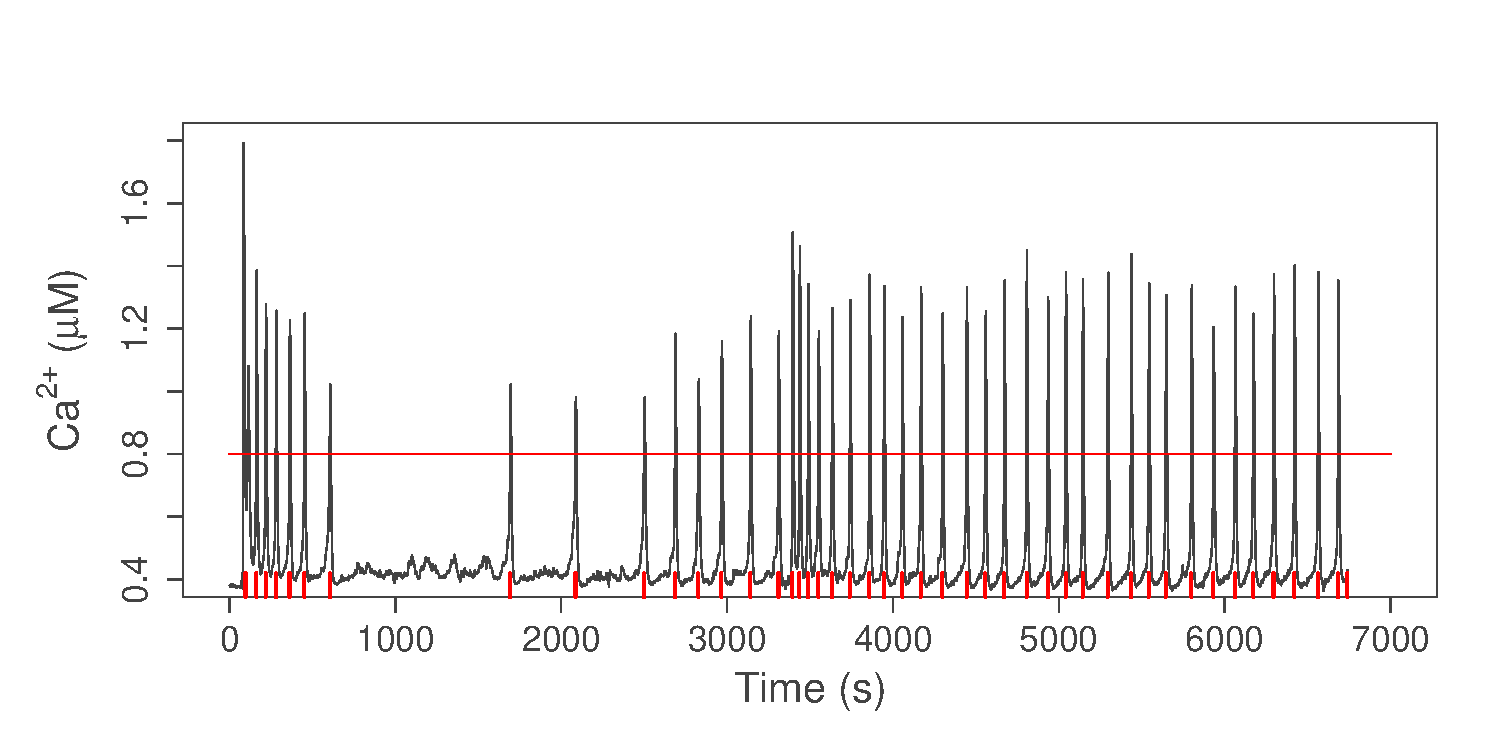
\includegraphics[scale = 0.45]{Trace} }} 
 
    \end{center}     
    \caption{Fura-2 fluorescence intensity traces of a HEK293 cell stimulated initially by 20$\mu$M carbachol and then with 50$\mu$M carbachol at 3444s. Where spike times (red rugs) are recovered by thresholding (red line) the concentration values at 0.8$\mu$M. (Data taken from M Falcke for experiment details see \cite{Thurley_2014} )  }
     \label{fig:trace}
    \hrulefill
    \end{figure}
    
Before we create a model for \ce{Ca^2+} spiking in cells, we first need to understand the raw data received from experimentalists. The raw data consists of time-series data for concentration of calcium in an individual cell, such as the black trace plot in figure \ref{fig:trace}, from which we can see the transient rises and falls in the \ce{Ca^2+} concentration. We then transform the data into a series of spikes by thresholding  the calcium concentration (red line in figure \ref{fig:trace}) and obtain the spike times (red rugs on x-axis). This is shown for one cell, however we have data from a variety of cells (HEK293, HeLa, Astrocyte, etc) under different stimuli. Hence our aim is to create a model to mimic the behaviour of \ce{Ca^2+} spikes in cells, and create simulated data, in addition to fitting the model to individual cells and recovering the spiking rate and spike variance. Once we fit the model, we can ask questions such as, could we infer what type of cell or stimulus strength was used in the experiment? 
    
A natural starting point to model \ce{Ca^2+} spikes are point processes, where each spike is an event in the process. Point processes are fully defined by their inter-event distribution, or in our case inter-spike interval (ISI) distribution. Namely, the probability $p(s,t)$ of a spike occurring at time $t$ given that the last spike occurred at time $s$, i.e spikes occur at times $s$ and $t$ with no spikes in the interval $(s,t)$. ISIs are obtained directly from experimental recordings, from which we can acquire the empirical distribution. From this we can choose a probability distribution to model the ISI, such as the Gamma, Weibull, inverse Gaussian distributions.  For example the probability density function of the Gamma distribution is
\begin{equation}\label{eq:1}
p(s, t | \alpha, \beta) = \frac{\beta^\alpha}{\Gamma(\alpha)} (t-s)^{\alpha-1} e^{-\beta (t-s)}, 
\end{equation}
where $\alpha$ and $\beta$ are the shape and rate parameters respectively and $\Gamma$ denotes the Gamma function. Research has shown that directly after a spike in \ce{Ca^2+} concentration the probability of a spike occurring shortly afterwards is low \cite{Thurley_2011}. The downtime after a spike when no spikes occur is known as the refractory period $t_{\mathrm{refract}}$.   The Gamma distribution is a suitable choice since increasing both $\alpha$ and $\beta$ simultaneously, whilst retaining the ratio $\alpha / \beta$, has the affect of maintaining the mean of the distribution but decreasing the variance, which will in turn reduce the probability of a spike occurring in the refractory period. Another approach would be to directly incorporate the refractory period into the ISI probability density, i.e add a parameter $t_{\mathrm{refract}}$ such that if $t < t_{\mathrm{refract}}$ then $p(s,t) = 0.$ This is done with the exponential distribution in \cite{Skupin}. The advantage of this approach is that since we assume spikes ISIs are independent and identically distributed the probability of an entire sequence of spikes factorises into individual ISIs. Suppose \ce{Ca^2+} spikes occur at times $y_1, y_2, \dots y_n$ and denote the set of all spikes by $\mathbf{y}$. Then the probability density of the spikes sequence factorises to
\begin{equation}\label{eq:2}
p(\mathbf{y}) = p_1(0,y_1)p(y_1,y_2) \dots p(y_{n-1},y_{n}) p_n(y_n,T),
\end{equation}
where $p_1(0,y_1)$ denotes the probability density of the first spike occurring at time  $y_1$ and $p_n(y_n,T)$ denotes the probability density of no spikes occurring between $y_n$ and the end of experiment time $T$. These events are separated as they do not constitute an ISI, and as such they are often modelled by different probability distributions, such as an exponential. 

These models are often referred to as stationary, since the ISIs have identical distributions. Moreover, the ISI probability depends only on the time since the last spike and not on the absolute experiment time. For example, suppose the first two spikes are separated by 100s, the probability of this occuring is the same whether the first spike occurs 50s or 1000s into the experiment. From figure \ref{fig:trace} we notice that after the stimulus is exchanged the rate of spiking increases (approximately at 3500s), in this instance it appears that the spiking rate depends on the absolute time of the experiment. Furthermore, there are numerous biological reasons why the ISI probabilities do not remain constant over time (see chapter {\it intro}). 

Thus we seek a method to mathematically describe the non-stationarity of the ISIs. One approach would be to add an explicit time-dependence into the ISI distribution by making the ISI parameters vary with time. However, the probability of a spike sequence need not factorise as \eqref{eq:2}, and we would have to consider the full multivariate probability density $p(\mathbf{y}) = p(y_1, \dots,y_n)$, which can present substantial difficulties.

A more practical approach was used by Barbieri et al in 2001 \cite{IntFn} via a time-rescaling method which maps the original experiment time $t$ to a new time $z$ by 
\begin{equation}\label{eq:3}
z(t) = \int^t_0 x(\nu ) d\nu, 
\end{equation}
where $x(\cdot)$ is called the intensity function, and is strictly positive. Since $x(\cdot)$ is positive it associates each $t$ with a unique value of $z$. The intensity encompasses the history dependence, and once rescaled in time $z$ the ISIs become independent, which allows the spike sequence to factorise into individual ISI contributions 
\begin{equation}\label{eq:4}
p(\mathbf{y} | x) = g_1(0, z_1)g(z_1, z_2) \dots g(z_{n-1},z_n) g_n(z_n, Z).
\end{equation} 
Where $z_i = z(y_i)$ and $Z = z(T)$ are the transformed spike times and experiment time respectively. We include the dependency on the intensity $x(t)$ directly to emphasise that the transformation depends on the intensity function. The probability density $g$ relates to the original ISI probability density $p$ by 
\begin{align} \label{eq:5}
g(z_i,z_{i+1} | x) =& \frac{dz}{dt} \bigg\rvert_{y_{i+1}} p(z_i, z_{i+1}),  \\
=& x(y_{i+1}) p(z_i, z_{i+1}). \label{eq:5b}
\end{align}

To illustrate this with the Gamma ISI distribution we begin with the one-parameter Gamma with mean 1, and denote its parameter by $\gamma$. The probability density of a spike occurring at time $y_i$ given the last spike occurred at $y_{i-1}$ is
\begin{equation} \label{eq:6}
p(y_{i-1}, y_i | \gamma) = \frac{\gamma ^\gamma}{\Gamma (\gamma )} (y_i-y_{i-1})^{\gamma - 1}  e^{-\gamma \left( y_i-y_{i-1} \right) }.
\end{equation}

 Subsituting \eqref{eq:6} into \eqref{eq:5b} gives the new ISI probability density
 \begin{equation} \label{eq:7}
p(y_{i-1},y_i|x, \gamma) = \frac{\gamma x(y_i)}{\Gamma (\gamma)} \big[ \gamma X(y_{i-1},y_i) \big]^{\gamma - 1} \mathrm{e}^{-\gamma X(y_{i-1},y_i) },
\end{equation}
 where
 \begin{equation}\label{eq:8}
X(s,t) = \int^{t}_{s} x(u) du , \qquad \text{for any } s,t \in [0,T].
\end{equation}
 From now on we drop the notation that the probability density is denoted by $g$ in the transformed time and use $p$ throughout. 
At this stage, it may appear that the intensity $x(t)$ is devoid of biological meaning, and only a mathematical trick. However, in fact $x(t)$ corresponds to the spiking rate independent of spike history. An example is shown in section 2 (figure \ref{fig:rastor}B).

In summary, we model \ce{Ca^2+} sequences as point processes that are fully described by their ISI distribution, which requires distribution type (Gamma, Weibull, etc) with parameter $\theta$ and the intensity function $x(t)$. Above we have shown the case for the Gamma distribution, however the concept can be used for any probability distribution on $(0,\infty)$ used to describe the ISI dynamics.

Notice that the more complex time-heterogeneous model contains the simpler stationary model. To visualise this suppose that the intensity function is constant $x(t) = x^*$ for some $x^* > 0$, then the integrated intensity simplifies to $X(s,t) = x^*(t-s)$. Substituting this into \eqref{eq:7} we retrieve the simple Gamma distribution with shape $\alpha = \gamma $ and rate $ \beta = \gamma x^*$, in \eqref{eq:1}.  


%%%%%%%%%
%% Simulating Spike Sequences
%%%%%%%%%
\section{Simulating Spikes}
Suppose we are given the ISI distribution with parameter $\theta$ and the intensity function $x(t)$, our goal is to create spike sequences from the model. There are numerous ways to simulate spike sequences, such as time rescaling, an approach using a Bernoulli process and the inverse transform method \cite{rescale, Truccolo_2005, InvTrans}. For all ISI distributions bar the exponential we use the inverse transform method. Since the exponential distribution leads to an inhomogeneous Poisson process, we use a thinning method \cite{PP}. This method begins by simulating from the homogeneous Poisson process with rate $\max(x(t))$, and then thinning (removing) spikes with probability $x(y_i) / \max(x(t))$. 

The inverse transform method samples from the target distribution by initially sampling a number $a$ from the uniform distribution on $[0,1]$, interpreted as a probability. Then if the cumulative density function (CDF) $F$ of the target distribution is know, return $F^{-1}(a)$, the inverse CDF evaluated at $a$ . However, in our case the CDF does not have closed form. Hence we discretise time and numerically calculate the CDF. 

Thus to simulate spike sequences we require the inputs: time length of experiment $T$, the ISI distribution, ISI parameter $\theta$, intensity $x(t)$ defined on $[0,T]$ and the discretisation of time defined by the number of steps $K$. With $K$ steps the discretisation is defined by $\mathbf{t} = \{ t_i\}^K_{i=0}$ and $t_i = iT/K$. The method is described in Algorithm 1, where $C$ stores the value of the CDF whilst we iterate through times $t$ and $y_{\mathrm{cur}}$ stores the most recent spike time.         

\begin{algorithm}[t]
\DontPrintSemicolon
\textbf{Input:}\text{ $T$, $K$, ISI distribution, $\theta$ and $x(t)$.  }\\ 
\textbf{Output:}\text{ A spike sequence $\mathbf{y}$ between $[0,T]$. }\\
\vspace{0.3cm}
Set $t=0$, $y_{\mathrm{cur}} = 0$, $\mathbf{y} = \oldemptyset$ and $h = T/K$; \;
\While{$t < T$}{
	Draw $a \sim U(0,1)$ and set $C = 0$; \;
	\While{$C< a$}{
	$t = t+h$; \;
	\If{$t > T$}{
	STOP; \;
	}
	Numerically calculate $C$ $= \int^t_{y_{\mathrm{cur}}} p(y_{\mathrm{cur}}, u |x(u), \theta ) du$; \;
	}
	Add $t$ to the set of spike times $\mathbf{y}$, and set $y_{\mathrm{cur}} = t$; \;
}
\textbf{Return} spike times $\mathbf{y}$; \;
\caption{Simulating spike sequences.}
\end{algorithm}

 %Figure rastor and PSTH. 
  \begin{figure}[t]
   \hrulefill
   \begin{center} 
    \subfloat[]{{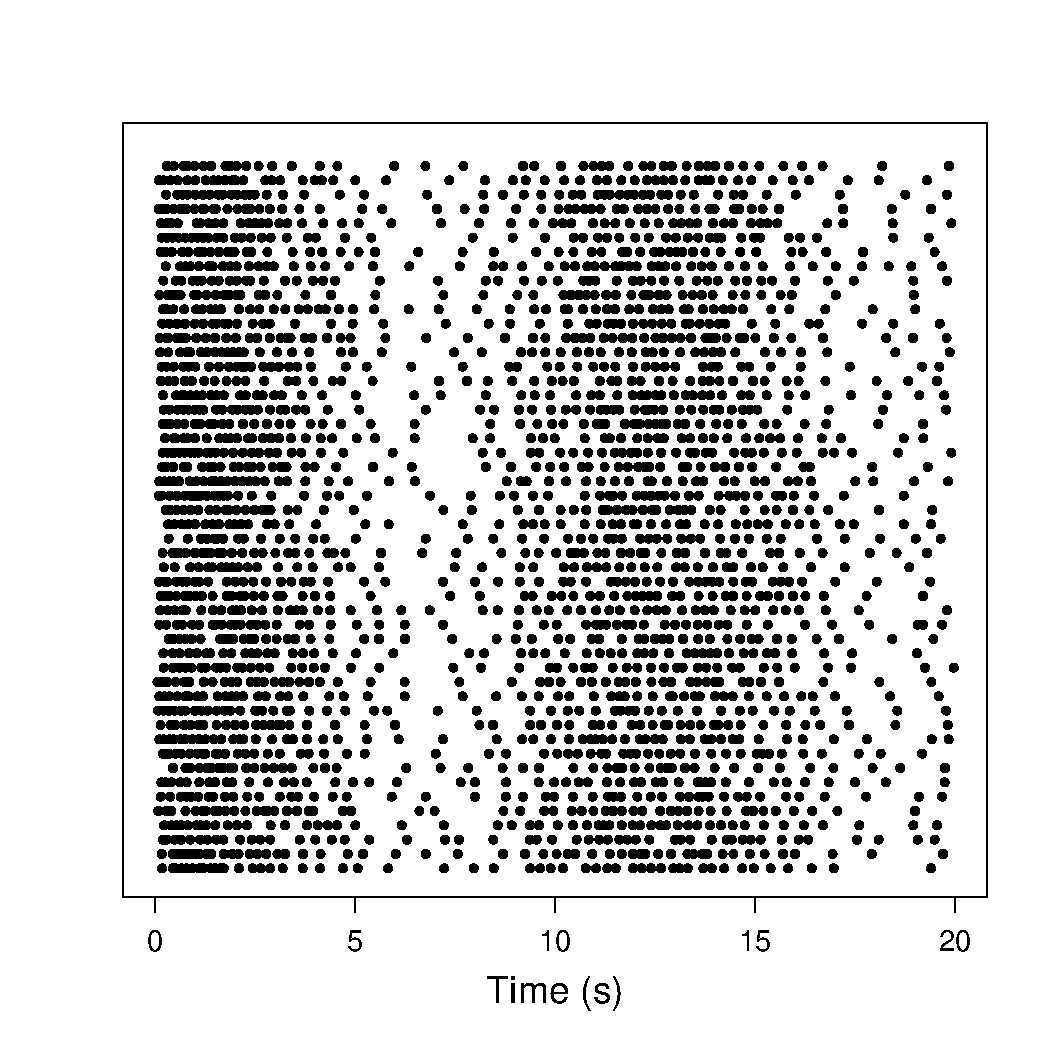
\includegraphics[scale = 0.36]{Rastor} }} \qquad
    \subfloat[]{{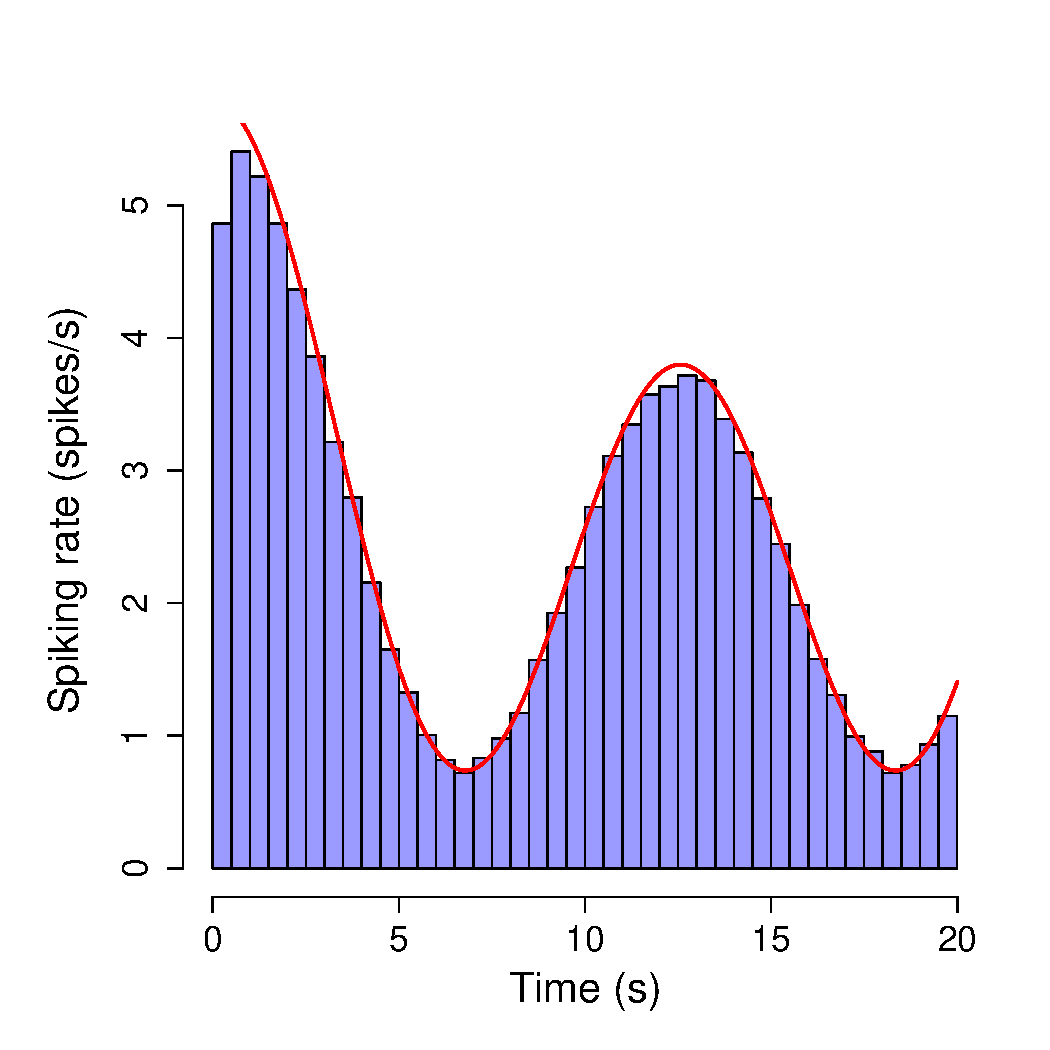
\includegraphics[scale = 0.36]{histogramSpikes} }} 
    \end{center}     
    \caption{ (A) Rastor plot of spikes simulated from a Gamma ISI distribution with parameter value $\gamma = 10$ and intensity function $x(t) = 2\cos\frac{t}{2} + \cos\frac{t}{4}+2.8$, between 0 and 20s. (B) Intensity function (red) alongside peristimulus-time histogram (blue) obtained from 1000 spike sequences simulated from the same distribution as (A).   }
     \label{fig:rastor}
    \hrulefill
    \end{figure}

%\begin{itemize}
%\item Draw a random number from the uniform distribution on the unit interval, $a \sim U(0,1)$.
%\item Since the cumulative density function does not have closed form for these distributions we numerically calculate
%\begin{equation}
%F(t|y_n, x, \theta) = \int^t_{y_n} p(y_n, u |x(u), \theta ) du,  
%\end{equation}
%with $t> y_n$.
%\item Generate spike times from
%\begin{equation}
%y_{n+1} =  \inf\{ t | F(t|y_n, x, \theta) > a \}.
%\end{equation}
%\end{itemize}
%
%Then $\{y_i\}^N_{i=1}$ are the resultant simulated spike times. \\

As stated previously, $x(t)$ is the spiking rate independent of the spike history. Hence, if we simulate a large number of spike sequences from the same distribution and then average over all of the sequences this should return the intensity function.  

In figure \ref{fig:rastor}A we have simulated 50 spike sequences from the model defined by the intensity function $x(t) = 2\cos\frac{t}{2} + \cos\frac{t}{4}+2.8$, with Gamma ISI distribution with parameter $\gamma = 10$. In figure \ref{fig:rastor}B using the same model we simulate 1000 sequences and binned the spikes (blue histogram). Since we used a large number of spike sequences this is equivalent to taking the average number of spikes across each small region, thus returning the expected number of spikes in each bin irrespective of the spike history. The strong agreement between the histogram and the intensity function (red line) confirms the interpretation of $x(t)$.  


%%%%%%%%%
%% Bayesian Inference
%%%%%%%%%
\section{Bayesian Inference }
We have shown that given some parameters for a cell spiking we can simulate spike sequences. Now consider the reverse question, if given spike data can we infer the model parameters from which the spikes occurred. Informally, what does the data inform us about the parameters of the model? Consider a single cell and observe its \ce{Ca^2+} concentration over the time period $[0,T]$. From this we determine the times $0< y_1 < \dots < y_N < T$ at which the \ce{Ca^2+} spikes occur. Let $\mathbf{y} = \{y_i\}_{i=1}^N$ denote the set of all spike times. Then the quantity of interest is the {\it posterior } distribution $\pi (x,\theta | \mathbf{y})$, which is the probability distribution of the parameters given the data. This approach has the benefit that we do not merely get a point estimate for our parameters but a joint distribution of $x$ and $\theta$. 

Consider the distribution for $\theta$ the ISI parameter. If the distribution is strongly centred around the value $\theta^*$ then we can be confident that $\theta^*$ is a good estimate for $\theta$. However, picture a distribution with multiple maxima or large variance, this would imply less confidence in the estimate.  This is an advantage of distributions over point estimates. 

Furthermore, the  joint posterior distribution is all we need to answer any question about the experiment or model dynamics, such as mean, variance or the interplay between ISI parameter and intensity function.  
 
To calculate the posterior distribution we apply Bayes' theorem

\begin{equation}\label{eq:Bayes}
\pi (x, \theta |\mathbf{y}) = \frac{ \pi(\mathbf{y} | x, \theta)  \pi(x, \theta)}{ \pi(\mathbf{y})}.
\end{equation}

On the right hand side we have: the likelihood function $ \pi(\mathbf{y} | x,\theta)$, the prior $\pi(x, \theta)$ and the normalising constant  $\pi (\mathbf{y})$.

  We need to derive an expression for the likelihood in our model. In our case this means the likelihood of obtaining the spike sequence given the parameters of the model, i.e. the probability of spike sequence $\mathbf{y}$ given $x(t)$ and $\theta$. This is exactly how we defined the model in section 1.1 (see \eqref{eq:4} and \eqref{eq:5b}), and as such the joint probability density of a spike sequence factorises into individual ISIs. Thus, the likelihood is given by
\begin{equation} \label{eq:10}
\pi(\mathbf{y} |x, \theta) = p_1(y_1|x) p_T(T,y_N|x) \prod^N_{i=2} p(y_{i-1},y_i|x, \theta).
\end{equation} 

Here, $p_1(y_1|x)$ represents the conditional probability of finding the first spike at time $y_1$. Furthermore, $p_T(T,y_N|x)$ represents the conditional probability of finding no spike in the interval $(y_N, T]$. We assume $p_1$ and $p_T$ come from an inhomogeneous Poisson process, i.e.

\begin{equation} \label{eq:11}
p_1(y_1|x) = x(y_1)e^{-X(0,y_1)} , \qquad p_T(T,y_N|x) = e^{-X(y_N,T)}, 
\end{equation}
 
 where $X(\cdot,\cdot)$ comes from \eqref{eq:8}.

For the Gamma ISI distribution putting together equations \eqref{eq:7}, \eqref{eq:10} and \eqref{eq:11} gives the likelihood to be

\begin{multline}\label{eq:fulllikeli}
\pi(\mathbf{y} | x, \gamma) = x(y_1) e^{-X(y_0,y_1)} e^{-X(y_N,T)}  \\
 \times  \prod^N_{i=2}  \frac{\gamma x(y_i)}{\Gamma ( \gamma )} \big[ \gamma X(y_{i-1} , y_i ) \big]^{\gamma -1} \exp( - \gamma X(y_{i-1} , y_i )  ).
\end{multline}

The {\it prior} contains our beliefs about the parameters before seeing the data. For example, if we strongly believed  $\theta$ to be close to the value $\theta^*$ then we would choose a prior distribution that is centred around $\theta^*$, such as $\pi(\theta) =$ Gamma$(\kappa \theta^*, \kappa )$ for some value of $\kappa$. On the other hand, if we are unsure of the value of $\theta$ we would choose a wider prior. Moreover, if we believe there is a positive correlation between say $\theta_1$ and  $\theta_2$ then a priori we could choose a  joint distribution with positive correlation such as the bivariate normal, $\pi (\theta_1, \theta_2) = \mathcal{N} \left( \left( \theta_1^* , \theta_2^* \right), \Sigma \right)$, where $\Sigma$ has positive correlation. 

It is easy to think of priors for ISI parameter $\theta$ as this is just a point variable, however it is harder to imagine a prior for the function $x(\cdot)$. We require a prior over the space of functions on $[0,T]$. The first method to combat this is to add a parametric form to $x(t)$, the most basic of which would be to assume it is constant, $x(t) = x$. This simplifies the problem greatly and a distribution on $(0,\infty)$ would suffice. To allow for time-heterogeneity more complex forms could be considered,  such as a quadratic $x(t) = at^2 + bt + c$. Then to describe our model we would need priors on $\{a,b,c\}$, such as independent Gamma distributions. However, even with this improvement over the constant intensity, we are still limited to what shape $x(t)$ takes. Furthermore, a priori there is little evidence to suggest what parametric form $x(t)$ takes, and this could vary significantly from cell to cell. 

Hence, we aim to use a non-parametric method for the prior as this allows more freedom on the shape that $x(t)$ can take. We use two such methods, namely applying a Gaussian Processes (GP) - as suggested by Cunningham et al in 2008 \cite{Cunningham2008} and a piecewise constant (PWC) prior. Details of how these priors work are in the subsequent sections 1.4.3 and 1.4.2 respectively.

Expanding the normalising constant we have
\begin{equation}
\pi(\mathbf{y}) = \int \pi(\mathbf{y} | x, \theta) \pi(x, \theta) dx d\theta,
\end{equation} 

which is an integral over all intensity functions and $\theta$. The high dimensionality of this integral would require efficient methods, as a direct integration would be computationally expensive if not impossible. Rather than compute the posterior directly, Tituaine et al  in 2017 \cite{AGNE:1} determined the maximum of the distribution and its variance, by applying Laplace's approximation for the intensity and integrating out the ISI parameter . Whilst this is a sufficient method it does has its limitations, since it only approximates the intensity function. %Furthermore, the integration used to remove the ISI parameter was dependent on discretised grid.
 We adopt a different approach using Markov chain Monto Carlo (MCMC). The computational difficult part of the posterior calculation comes from the normalising constant. Thus, MCMC samples from $p(x,\theta | \mathbf{y})$, where we only need to know the distribution up to a multiplicative constant. Then from the samples we recover the possible values and their associated probabilities, without having to calculate a closed form solution. This is due to the fact that if a value is more likely then it will get sampled more often.  
The construction of the MCMC algorithms are detailed in the next section.

The method above can be generalised to input multiple spike sequences. Assuming the multiple spike sequences $\{\mathbf{y}^i \}^M_{i=1}$ are all independent then the only effect is on the likelihood, where we now have the product of all the individual spike sequences
\begin{equation}
\pi \left( \left\{\mathbf{y}^i \right\}^M_{i=1} | x, \theta \right) = \prod^M_{i=1} \pi \left( \mathbf{y}^i | x, \theta \right),
\end{equation} 
Multiple spike sequences may be considered if we believe the spikes all come from the same distribution.


%%%%%%%%%
%% BAYESIAN COMPUTATION
%%%%%%%%%
\section{Bayesian Computation}
In this section we explore how to use MCMC methods to obtain the posterior distribution of the model parameters. The concept behind MCMC is that if the required probability density is know up to a multiplicative constant, then we can create a Markov chain whose stationary distribution is the probability density we desire. Once we create the chain, we start at some arbitrary initial value and iterate the Markov chain to create samples. Doing so many times, the samples converge onto the target stationary distribution. There are many standard MCMC methods (e.g Gibbs sampler, Metropolis-Hastings Algorithm \cite{Gibbs, Hastings}), which can be used in a plethora of different problems. However, due to the fact that the intensity is a function of time we will require complex MCMC algorithms to sample from the desired posterior.

In layman's terms, an MCMC algorithm begins at some initial value, say $\phi_0 = \phi_0$ where $\phi$ can be and often is multi-dimensional. Suppose we are at iteration $i$, where the current value is $\phi_i$, we have a proposal regime that gives us a new candidate value $\phi^*$, often dependent on the current value $\phi_i$.  Then we accept the candidate value with probability $p_\mathrm{acc}$, relating to the probability that $\phi^*$ is a better estimate then $\phi_i$, giving $\phi_{i+1} = \phi^*$, else $\phi_{i+1} = \phi_i$.

We utilise a Gibbs sampling method over $x(t)$ and  ISI parameter $\theta$. This means that rather then propose candidate values of both parameters together, we split the algorithm into two sections where  we update $x(t)$ first and then update $\theta$.  So rather then sample from the full joint distribution we sample from the conditional distributions. One benefit of this method is that the conditional distributions are often easier to deal with then the full joint distribution. 
The MCMC algorithm begins by choosing initial values $x_0$ and $\theta_0$ then iterating the process 

\begin{steps}
\item Update the $x(t)$ applying either piecewise constant prior (section 1.4.2) or Gaussian Process prior (section 1.4.3);
\item Update $\theta$ using a Metropolis-Hastings algorithm  (section 1.4.4).
\end{steps}

Thus the algorithm returns samples for $x$ and $\theta$, namely $\{x_i \}^M_{i=1}$ and $\{\theta_i \}^M_{i=1}$, where $M$ is the total number of iterations. It often takes the algorithm time to converge onto the target distribution, as such the first $M_{\mathrm{burn}}$ iterations are removed. 

However, we begin in the next section by applying MCMC methods to the case $x(t)$ is constant. This significantly reduces the difficultly of the problem, nevertheless it is a good starting point and is useful to compare with the time-dependent models later.

%%%%%%%%%
%% Simple (intensity fixed)
%%%%%%%%%
\subsection{Simple Model}
We begin by assuming the intensity function is constant, $x(t) = x$. As stated previously, this assumption gives rise to time-homogeneity. Furthermore, we get $X(s,t) = x(t-s)$ for the integrated intensity function in the likelihood. The model is now simpler as we only need to estimate two parameters, $x$ and the ISI parameter $\theta$. We use two different methods to achieve this, Maximum likelihood estimation (MLE) and MCMC. 

We need to decide prior distributions for $x$ and $\theta$, we choose to use Independent Gamma distributions for both $x$ and $\theta$, i.e. 
\begin{equation}\label{eq:SimPrior}
\pi(x) = \Gamma(\alpha_x, \beta_x) \quad \text{ and } \quad \pi(\theta) = \Gamma(\alpha_\theta, \beta_\theta).  
\end{equation}
These Gamma distributions are often set to be non-informative with shape 1 and rate small. If we assume the ISIs follows a Gamma distribution then the likelihood simplifies to
\begin{multline}\label{eq:likeliFixed} 
\pi(\mathbf{y} | x,\theta) =  x e^{-x(y_1-y_0)} e^{-x(T-y_N)}  \\
 \times  \prod^N_{i=2}  \frac{\gamma x}{\Gamma ( \gamma )} \big[ \gamma x(y_i - y_{i-1} ) \big]^{\gamma -1} \exp( - \gamma x(y_i - y_{i-1} )  ).
\end{multline}

MLE is a method where we search the parameter space and return the values which give rise to the largest likelihood. This is done using a classical optimiser function (such as {\it optim} in R), and returns a point estimate. The benefit of this method is that it is quick and easy to implement. However, it only returns individual values for the parameters, rather than full distributions. 
For example suppose we have spikes $\mathbf{y}$ and we want to fit the Gamma ISI distribution. MLE method works by solving for
\begin{equation}
(x^*, \gamma^*) =  \max_{x, \gamma \in \left(0, \infty \right)} \pi (\mathbf{y} | x, \theta), 
\end{equation}
where $\pi (\mathbf{y} | x, \theta)$ comes from \eqref{eq:likeliFixed}.
 
For the MCMC method we use Gibbs sampling. We use random walk (RW)-Metropolis algorithms to update $x$ and $\theta$ separately. The RW-Metropolis algorithm is a special case of the Metropolis-Hastings algorithm that comprises of two steps: a proposal regime and whether to accept the proposal. Suppose at our current iteration we have a value $z$ of the parameter of interest. We propose a new value $z'$ using the proposal distribution $q(z' |z)$ which is the conditional probability of proposing state $z'$ given we are in state $z$. Then we accept $z'$ with probability
\begin{equation}\label{eq:MH}
p_{\mathrm{acc}} = \min \left\{ 1,\frac{P(z') q(z |z')}{P(z) q(z' |z)} \right\},
\end{equation}    
where $P(z)$ is proportional to the target distribution (likelihood and prior). For RW-Metropolis the proposal distribution is Gaussian centred around the current value with variance given, $z' \sim N(z,\sigma)$. In this case the $q$ ratio in the acceptance probability cancels leaving
 \begin{equation}
p_{\mathrm{acc}} = \min \left\{ 1,\frac{P(z') }{P(z)} \right\}.
\end{equation}  



 %Figure for the simple model
   \begin{figure}[t]
   \hrulefill
   \begin{center} 
    \subfloat{{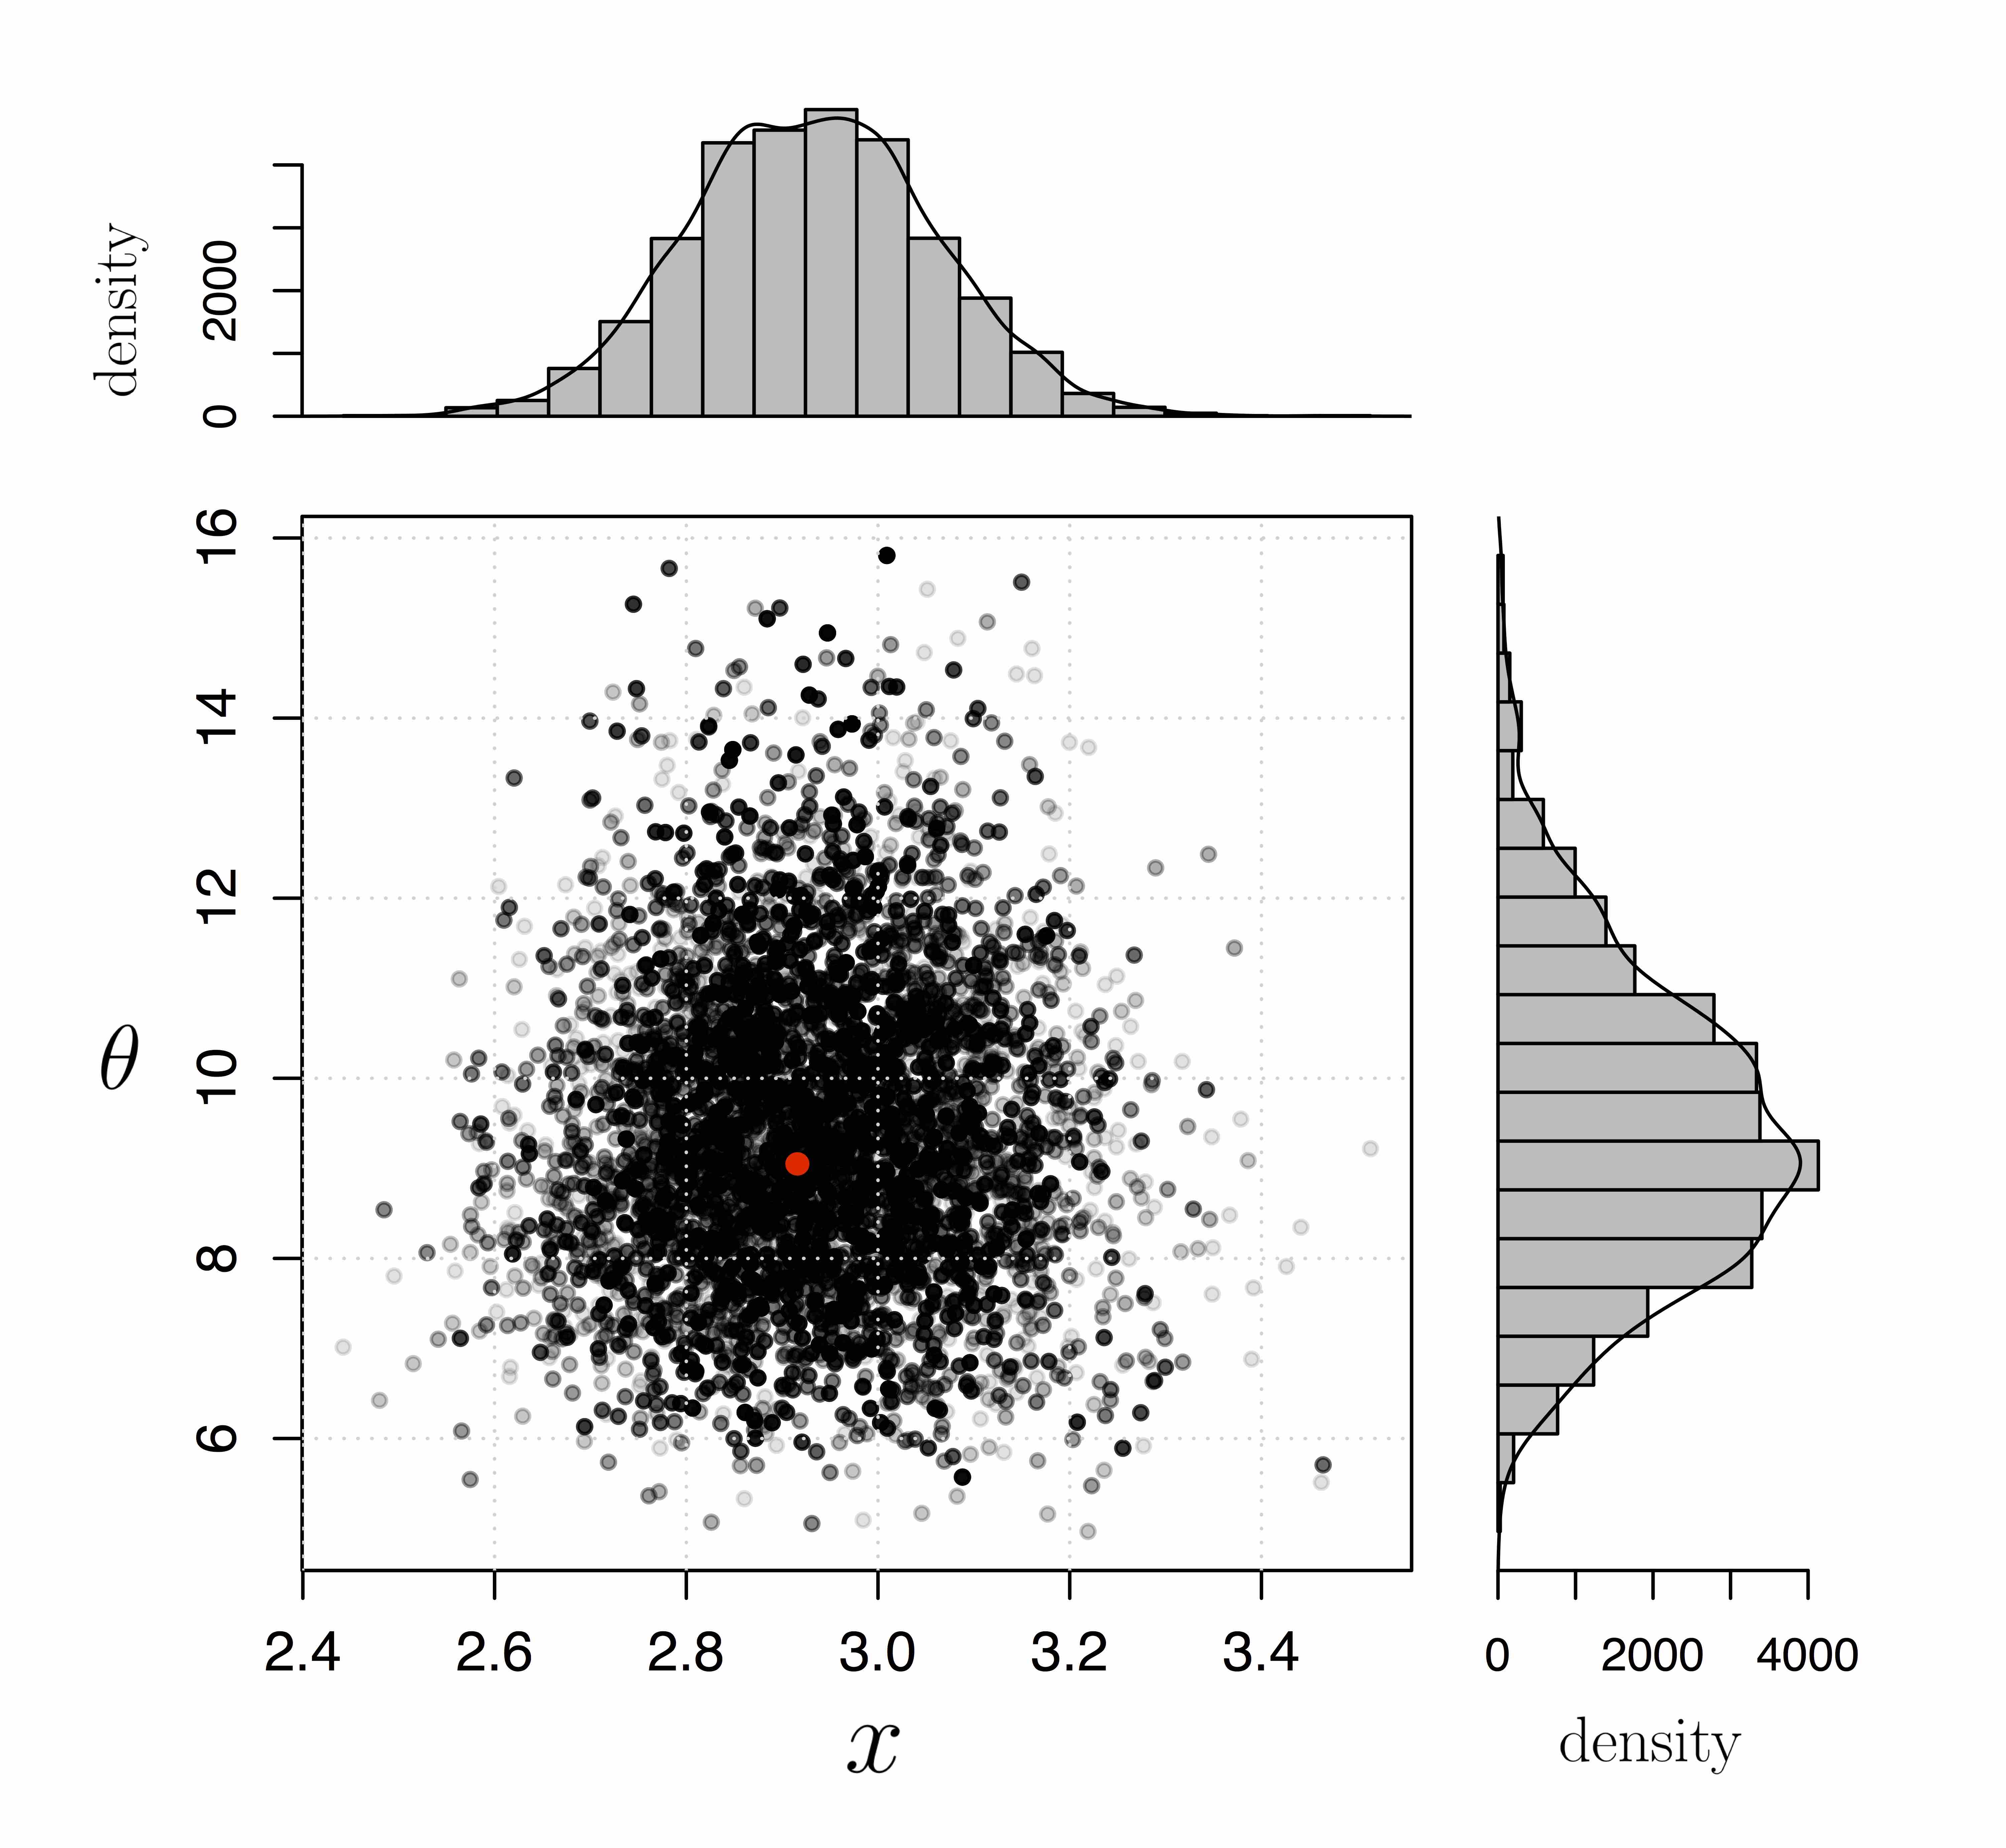
\includegraphics[scale = 0.04]{Simple} }}
    \end{center}     
    \caption{Posterior results from the simple model. Each grey point represents one sample from the posterior distribution, where overlapping values become darker. The red dot is the value obtained using MLE. The histograms, top and right, represent the individual posterior distributions of $x$ and $\theta$ respectively.  }
    \label{fig:simple}
    \hrulefill
    \end{figure}
 
 We now explain how to use this framework, within a Gibbs sampler to sample from ($x,\theta$). Since we update $x$ and $\theta$ separately, when updating $x$ $\theta$ is constant and vice versa. Hence the target distribution reduces to the conditionals $\pi(x | \theta, \mathbf{y})$ and $\pi(\theta | x, \mathbf{y})$  and by using Bayes' theorem
\begin{equation}
\pi(x | \theta, \mathbf{y}) = \pi(\mathbf{y}|x,\theta) \pi(x)   \quad \text{ and } \quad \pi(\theta | x, \mathbf{y}) = \pi(\mathbf{y}|x,\theta)
\pi(\theta). 
\end{equation}   
The algorithm begins by selecting initial values $x_{\mathrm{cur}} = x_0$ and $\theta_{\mathrm{cur}} = \theta_0$, sampling variances $\sigma^2_x$ and $\sigma^2_{\theta}$ and the number of iterations $M$. In each iteration, begin by updating $x$. Propose a new value $x_{\mathrm{can}} \sim N(x_{\mathrm{cur}}, \sigma^2_x)$, and accept the candidate value with probability $\min \left(1,\frac{\pi(x_{\mathrm{can}} |\theta_{\mathrm{cur}}, \mathbf{y})}{\pi(x_{\mathrm{cur}}|\theta_{\mathrm{cur}}, \mathbf{y})}\right)$. Next we update $\theta$ by proposing a new value $\theta_{\mathrm{can}} \sim N(\theta_{\mathrm{cur}}, \sigma^2_\theta)$, and it is accepted probability $\min \left(1,\frac{\pi(\theta_{\mathrm{can}} | y, x_{\mathrm{cur}})}{\pi(\theta_{\mathrm{cur}} | y, x_{\mathrm{cur}})}\right)$. Often the calculations include large powers of variables, for example the Gamma ISI distribution \eqref{eq:fulllikeli} contains $\gamma^\gamma$, where $\gamma$ can be large. To circumvent this issue the calculations are assessed on the logarithmic scale. The algorithm outputs a matrix of dimension $2 \times M$, where column $i$ contains the values $(x_i,\theta_i)$ the $i$th sample. Often, the initial $M_{\mathrm{burn}}$ iterations are removed to allow the Markov chain time to converge onto the stationary distribution.


In particular for the Gamma ISI distribution with parameter $\gamma$, we have the likelihood given by \eqref{eq:likeliFixed}. Expanding the priors for $x$ and $\theta$ in \eqref{eq:SimPrior} we have
%first calculate the likelihood by substituting $x(t) = x$ into \eqref{eq:fulllikeli}
%\begin{equation}
%\pi(\mathbf{y} | x, \gamma) = x e^{-x(y_1 -0)} e^{-x(T - y_N)} \prod^N_{i=2}  \frac{(\gamma x)^\gamma}{\Gamma ( \gamma )} \big[(y_i - y_{i-1} ) \big]^{\gamma -1} \exp( - \gamma x(y_i - y_{i-1} )   ).
%\end{equation}
\begin{equation}
\pi (x) = \frac{{\beta_x}^{\alpha_x}}{\Gamma \left( \alpha_x\right)} x^{\alpha_x - 1} \exp \left\{ - \beta_x x \right\} \text{  and  }
\pi(\gamma) = \frac{{\beta_\gamma}^{\alpha_\gamma}}{\Gamma \left( \alpha_\gamma\right)} \gamma^{\alpha_\gamma - 1} \exp \left\{ - \beta_\gamma \gamma \right\}.
\end{equation}

Recall we only require the density up to a multiplicative constant hence removing constants and rearranging we get the acceptance probability for $x$
\begin{align}
p^x_{\mathrm{acc}} &= \frac{x_{\mathrm{can}}^{\alpha_x} \exp\left\{-x_{\mathrm{can}} \left(\beta_x + y_1 +(T-y_N) \right)  \right\} \prod^N_{i=2}  x_{\mathrm{can}}^\gamma \exp( \left\{- \gamma x_{\mathrm{can}}(y_i - y_{i-1}) \right\} }
{x_{\mathrm{cur}}^{\alpha_x} \exp\left\{-x_{\mathrm{cur}} \left(\beta_x + y_1 +(T-y_N) \right)  \right\} \prod^N_{i=2}  x_{\mathrm{cur}}^\gamma \exp( \left\{- \gamma x_{\mathrm{cur}}(y_i - y_{i-1}) \right\}}, \\
 &=  \frac{x_{\mathrm{can}}^{\alpha_x +(N-1)\gamma} \exp\left\{-x_{\mathrm{can}}\left(\beta_x + y_1 +(T-y_N)  + \gamma \left(y_N-y_1 \right) \right)  \right\} }
 {x_{\mathrm{cur}}^{\alpha_x +(N-1)\gamma} \exp\left\{-x_{\mathrm{cur}}\left(\beta_x + y_1 +(T-y_N)  + \gamma \left(y_N-y_1 \right) \right)  \right\}}, \label{eq:12}
\end{align}
where $\gamma$ is equal to the current value at the start of the iteration. In the case of the Gamma ISI distribution it is possible to simplify the method stated above. Note that the conditional $\pi(x | \gamma, \mathbf{y})$ (i.e the numerator in \eqref{eq:12}) is the kernel of a Gamma distribution. This implies that when we update $x$ we can draw from distribution $\Gamma \left( \alpha_x +(N-1)\gamma, \beta_x + y_1 +(t-y_N)  + \gamma \left(y_N-y_1 \right)  \right)$. However, we use  RW-Metropolis for $x$ here as this is required for other ISI distributions.

Similarly the acceptance probability for $\gamma$ is
\begin{align}
p^\gamma_{\mathrm{acc}} &= 
 \frac{{\gamma_*}^{\alpha_\gamma - 1} e ^{-\beta_\gamma {\gamma_*}} \prod^N_{i=2}  \frac{({\gamma_*} x)^{\gamma_*}}{\Gamma ( {\gamma _*} )} \big[(y_i - y_{i-1} ) \big]^{{\gamma _*} -1} \exp( - {\gamma _*} x(y_i - y_{i-1} )   )}
 {\gamma^{\alpha_\gamma - 1} e ^{-\beta_\gamma \gamma} \prod^N_{i=2}  \frac{(\gamma x)^\gamma}{\Gamma ( \gamma )} \big[(y_i - y_{i-1} ) \big]^{\gamma -1} \exp( - \gamma x(y_i - y_{i-1} )   )}, \\
 &=  \frac{\gamma_*^{\alpha_\gamma - 1} \exp \left\{ -\gamma_* \left( \beta_\gamma + y_n-y_1 \right) \right\} 
 \frac{(\gamma_* x)^{(N-1)\gamma_*}}{\Gamma ( \gamma_* )^{N-1}}
 \prod^N_{i=2}  (y_i - y_{i-1} )^{\gamma_* -1}}
 {\gamma^{\alpha_\gamma - 1} \exp \left\{ -\gamma \left( \beta_\gamma + y_n-y_1 \right) \right\} 
 \frac{(\gamma x)^{(N-1)\gamma}}{\Gamma ( \gamma )^{N-1}}
 \prod^N_{i=2}  (y_i - y_{i-1} )^{\gamma -1}},
\end{align}
where we swap notation $\gamma_{\mathrm{cur}} = \gamma$ and $\gamma_{\mathrm{can}} = \gamma_*$ for clarity in the equation, and $x$ is the current value in the iteration. Due the large number of exponents and exponentials the calculations are computed on the logarithmic scale.  We draw $u \sim U[0,1]$, then accept the candidate value if $\log u < \log p_{\mathrm{acc}}$.    
 
In figure \ref{fig:simple} we give an example for simulated data with 58 spikes generated between 0 and 20s, from the model defined by $x(t) = 3$ and $\gamma = 9$.  We apply the MCMC algorithm beginning with $x_0 = 1$ and $\gamma_0 = 1$ and both variances $\sigma_x, \sigma_\gamma$ also set to 1. We ran the algorithm for 40000 iterations and removed the first 10000. Each grey dot represents the values of a single iteration of the algorithm, such that if dots overlap the colour becomes darker. We also calculate the MLE which corresponds to the red point in the scatter plot. We see that we recover the model parameters well, with most of the density centred about the true values. Furthermore, the MLE occurs at approximately the values with the most probability from the MCMC as expected.
 
 %%%%%%%%%
%% Piecewise Linear Model
%%%%%%%%%
 \subsection{Piecewise Constant Prior }
 We now generalise the simple model, where the intensity function can now take multiple values via a step function. We assume that a priori the intensity function is piecewise constant (PWC) and is defined by the times (change points) where the intensity changes and the values of the intensity between these times (heights). This is a reasonable assumption to make in step-change experiments, where the stimulus is exchanged during the experiment. Moreover, if cells experienced a constant stimulation, it is reasonable to assume $x(t)$ remains constant over large periods but the value may change due to biological phenomena, such as a change in ER \ce{Ca^2+} load. Even if a priori we believe the intensity varies continuously, every continuous function can be approximated by a step function, taking the number of change points to be large.
  
To apply Bayesian inference we require a prior distribution over the space of PWC functions and require an MCMC method to sample form the posterior. Notice that with this functional form the number of parameters that describe the intensity function changes depending on the number of change points. For example if $x(t) = 1$, we have 0 change points and 1 height and a total of 1 parameter, whereas if $x(t) = 0.5$ if $t<20$ and $1.5$ otherwise, we have 1 change point and 2 heights and a total of 3 parameters. Hence we require an MCMC method which allows jumps between parameter spaces with varying dimensions. We implement a Reversible jump MCMC (RJMCMC) technique \cite{RJMCMC}, which extends standard MCMC to allow for parameter spaces of varying dimension. In our case, the sample space is $\mathcal{X} = \cup_k \mathcal{X}_k$, where $\mathcal{X}_k$ corresponds to the parameter space with $k$ change points and $k+1$ heights. The method works by either changing parameter space or parameter values in the current space at each iteration, full details are in the preceding section.  
 
 The advantage of this method compared to the Gaussian Process prior (see section 1.4.3) is that it requires less computational demand. However in vitro the belief is that cells are exposed to time varying (continuous) stimuli and the intensity function should inherit this behaviour, thus with PWC we can only approximate this continuous change with step functions. 
 
% PRIOR DISTRIBUTION.
 \subsubsection{Prior Distribution}
 We assume that the intensity function $x(t)$ on $[0,T]$ is a step function. Suppose that there are $k$ change points $0 = s_0 < s_1 < \dots < s_k < s_{k+1} =T$ and that the height on each interval $[s_j, s_{j+1})$ is $h_j$ for $j = 0,1, \dots k$. 
 Hence we have
 
 \begin{equation}
 x(t) = \sum^k_{j=0} h_j \mathbf{1}_{[s_j,s_{j+1})} (t).
 \end{equation}
 
 { \color{blue}We assume that a priori $k$ has a Poisson distribution with rate $\lambda$ conditioned on $k \leq k_{\mathrm{max}}$
 \begin{equation}\label{eq:Poiss}
 p(k) = \frac{\lambda^k e^{-\lambda}}{k!}  \bigg/ \sum^{k_{\mathrm{max}}} _{i=0}  \frac{\lambda^i e^{-\lambda}}{i!}.
 \end{equation}
  This means that the most likely number of change points is $\lambda$ and we limit the maximum number to be $k_{\mathrm{max}}$. Suppose we have $k$ change points $s_1, \dots, s_k$ a priori  they are distributed as the even-numbered order statistics of $2k+1$ points uniformly and independently distributed on $[0,T]$. To visualise imagine we were to simulate the position of the change points, we would sample $2k+1$ points in the interval $[0,T]$. Then order the points from smallest to largest to obtain $\left\{t_i \right\}_{i=1}^{2k+1}$, and set $s_i = t_{2i}$ for $i \in 1,\dots, k$.   This prior for the change points was used by Green (1995) to probabilistically penalise short intervals and improve the spacing of the change points. }
 
      %Figure of How to move in RJMCMC.
  \begin{figure}[t]
   \hrulefill
   \begin{center} 
    \subfloat[]{{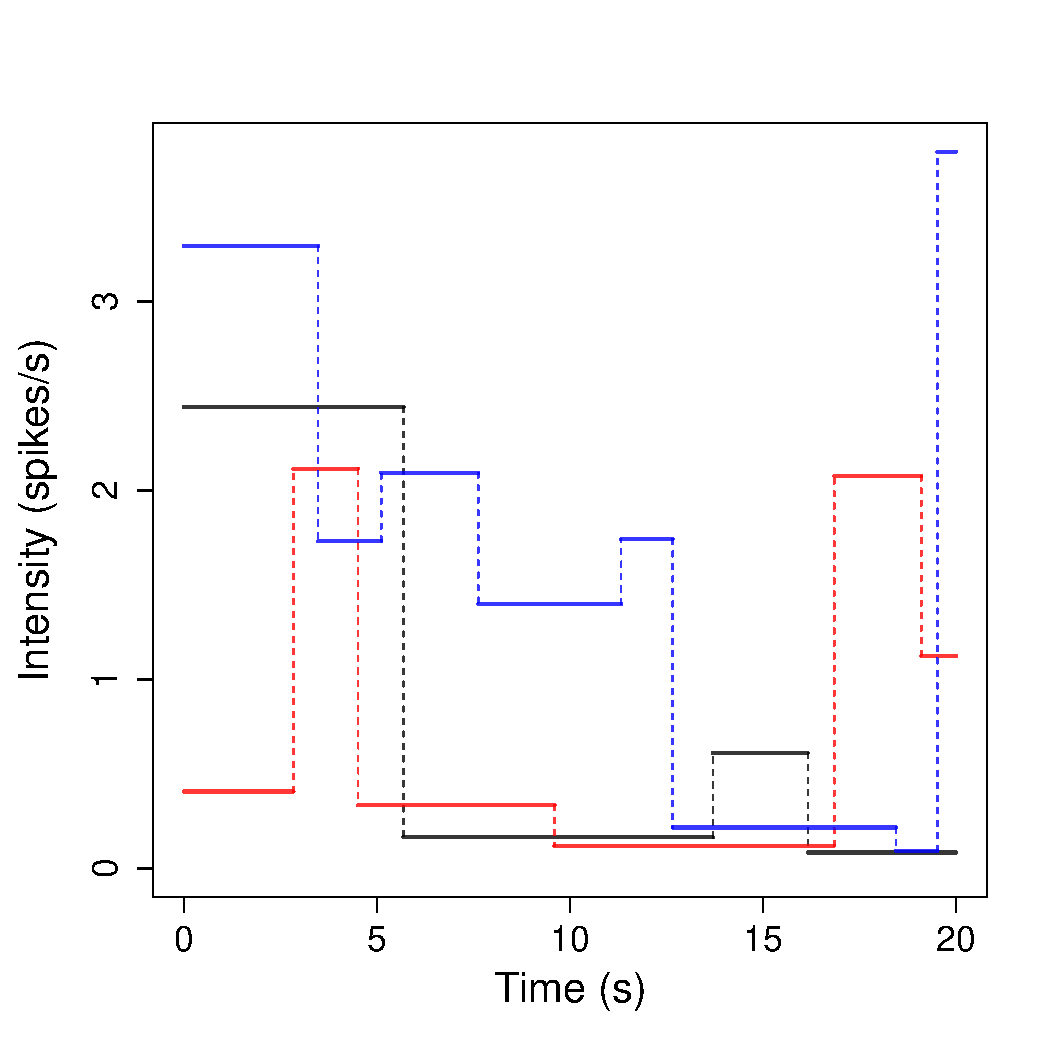
\includegraphics[scale = 0.36]{Draw_PW_Indep} }} \qquad
    \subfloat[]{{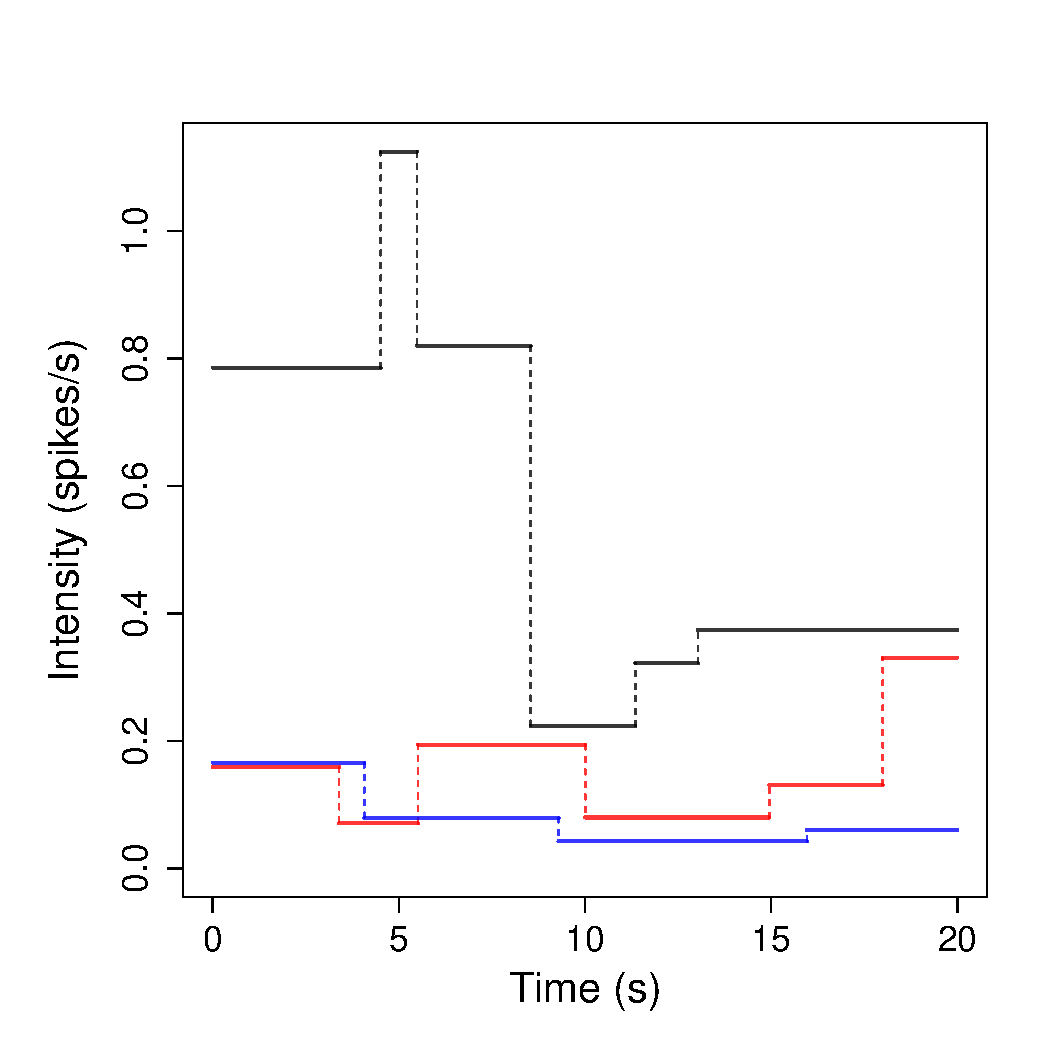
\includegraphics[scale = 0.36]{Draw_PW_Mart} }} 
    \end{center}     
    \caption{Realisations from the PWC prior. Where  $T = 20,  k_{\mathrm{max}} = 10, \lambda = 5, \kappa = 1$ and $\mu = 1$. In (A) the heights are independent and in (B) the heights follow the martingale structure.  }
    \hrulefill
    \label{fig:PWCDraw}
    \end{figure}
    
 For the heights we have two options for the prior. Firstly,  $h_0,h_1, \dots, h_k$ have independent $\Gamma (\kappa , \mu ) $ distributions.  Secondly, the heights can follow a martingale structure (Following Arjas and Gasbarra (1994) \cite{Martingale}) where we assume that $h_0 \sim $ Gamma$(\kappa, \mu)$ and that given $h_0, \dots h_{i-1},$ $h_i \sim$ Gamma$(\kappa, \mu_i)$ where $\mu_i = \kappa / h_{i-1}$ so that $\mathbb{E}[h_i | h_{i-1}] = h_{i-1}$. This should have the affect of smoothing $x(t)$. In Figure \ref{fig:PWCDraw} we see that the heights with the martingale structure do indeed vary less then those assumed to be independent.  Indeed, we see in figure 1.4 that with the martingale structure consecutive heights have more similar values than if the heights are assumed to be independent. 

    
    %POSTERIOR COMPUTATION.
 \subsubsection{Posterior Computation}
In this section we will show how the RJMCMC proposes new step functions, and whether or not to accept the new function.
In Algorithm 2 we have an outline of the MCMC algorithm where a priori the intensity function is PWC. Furthermore, the algorithm states when to update the ISI parameter, with more details in section 1.4.4. Note that the algorithm requires the following inputs: spikes $\mathbf{y}$; the ISI distribution (e.g. Gamma, Weibull. etc); the number of iterations to compute $M$ along with training period of $M_{\mathrm{burn}}$ iterations; the parameters of the PWC prior $\lambda, k_{\mathrm{max}}, \kappa, \mu$; the variance $\sigma^2_\theta$ used in the RW-Metropolis algorithm and the prior type for heights (either independent or martingale structure). It outputs M samples of x(t), where each sample is composed of position of change points and corresponding heights, where the number of change points and heights can vary in each sample.In addition to M samples of the ISI parameter $\theta$.    
 %-------- Algorithm. 
 \begin{algorithm}[t]
\DontPrintSemicolon
\textbf{Input:}\text{ Spikes $\mathbf{y}$, ISI distribution, $M$,$M_{\mathrm{burn}}$, $\lambda, k_{\mathrm{max}}, \kappa, \mu$, $\sigma^2_\theta$ and the }\\ 
\text{prior type for heights.} \\
\textbf{Output:}\text{ $M$ samples of the intensity $x(t)$, given by heights $\mathbf{h}$ and change }\\ \text{ points $\mathbf{s}$, and ISI parameter $\theta$.  }\\
\vspace{0.3cm}
Calculate $c$ such that $\max_k(b_k +d_k)=0.9$; \;
Set initial values $\mathbf{h}^{(0)}$, $\mathbf{s}^{(0)}$ and $\theta^{(0)}$; \;
\For{$i$ in 1 to $(M +M_{\mathrm{burn}})$}{
	Update the intensity function. \;  \Indp 
	Calculate $b_k$ and $d_k$; \;
	Draw $u \sim U(0,1)$; \;
		\textbf{(Step 1)} \If{$u <b_k$}{
			Propose a new change point and corresponding heights; \;
			Accept the proposed values with probability given by the acceptance probability, update $\mathbf{h}^{(i+1)}$ and $\mathbf{s}^{(i+1)}$ ; \;
		}
		\textbf{(Step 2)} \ElseIf{$b_k < u < b_k + d_k$}{
			Propose a death of a current change point and corresponding heights; \;
			Accept the proposed values with probability given by the acceptance probability, update $\mathbf{h}^{(i+1)}$ and $\mathbf{s}^{(i+1)}$; \;
		}
		\textbf{(Step 3)} \Else{
			Propose a move for an existing change point; \;
			Accept the proposed values with probability given by the acceptance probability, update $\mathbf{s}^{(i+1)}$; \;
			Propose a change of an existing height; \;
			Accept the proposed values with probability given by the acceptance probability, update $\mathbf{h}^{(i+1)}$;\;
		} \Indm
	Update the ISI parameter. \; \Indp
		Use RW-Metropolis algorithm to update $\theta$ (section 1.4.4); \;
		\Indm
			
}
Return $\mathbf{h}$, $\mathbf{s}$ and $\theta$ with initial $M_{\mathrm{burn}}$ iterations removed; \;
\caption{Inference for PWC prior.}
\end{algorithm}

 We will begin by considering the heights to be independent a priori, and discuss how the martingale structure alters the formulas afterwards.  At each iteration of the algorithm we make one of three types of updates:
\begin{enumerate}
\item Birth of a change point.
\item Death of a change point.
\item Within model updates (moving existing change points and change heights). 
\end{enumerate}

\noindent These occur respectively with probabilities $b_k, d_k$ and $ 1- b_k - d_k$, where

\begin{equation}
b_k = c \min\{1,p(k+1)/p(k) \}, \qquad \qquad d_k = c \min \{ 1, p(k-1)/p(k) \}.
\end{equation}

Above $p(k)$ is the probability mass function of a Poisson random variable with rate $\lambda$ conditioned with maximum value $k_{\mathrm{max}}$ and $c$ is chosen such that $\max_k (b_k +d_k ) = 0.9$ \cite{RJMCMC}. This is done to make sure within model changes occur at a frequent rate, such each iteration is not always a change in parameter space.\\

For all of the updates we need to calculate the likelihood ratio, i.e given the data the likelihood that the data comes from the given intensity function $x(t)$ and ISI parameter $\theta$. So suppose we initially have intensity function $x(t)$ and candidate intensity function is $x'(t)$ then 
the likelihood ratio is
\begin{equation}
\text{(likelihood ratio)} = \frac{\pi (\mathbf{y} | x', \theta)}{\pi (\mathbf{y} | x, \theta)}.
\end{equation}

Note that $\theta$ takes the same value in both numerator and denominator, thus any terms purely in $\theta$ cancel. In particular for the Gamma ISI distribution the likelihood function $p(\mathbf{y} | x, \theta)$ is given in \eqref{eq:fulllikeli}, with the ISI parameter becoming $\gamma$. This gives the ratio
\begin{equation}
 \frac{x'(y_1) e^{-X'(y_0,y_1)} e^{-X'(y_N,T)} \prod^N_{i=2}  x'(y_i) \big[ X'(y_{i-1} , y_i ) \big]^{\gamma -1} \exp( - \gamma X'(y_{i-1} , y_i )  )}
{x(y_1) e^{-X(y_0,y_1)} e^{-X(y_N,T)} \prod^N_{i=2}  x(y_i) \big[ X(y_{i-1} , y_i ) \big]^{\gamma -1} \exp( - \gamma X(y_{i-1} , y_i )  )},
\end{equation}
where $X'$ is the integrated candidate intensity function.\\

%Figure of How to move in RJMCMC.
  \begin{figure}[t]
   \hrulefill
   \begin{center} 
    \subfloat{{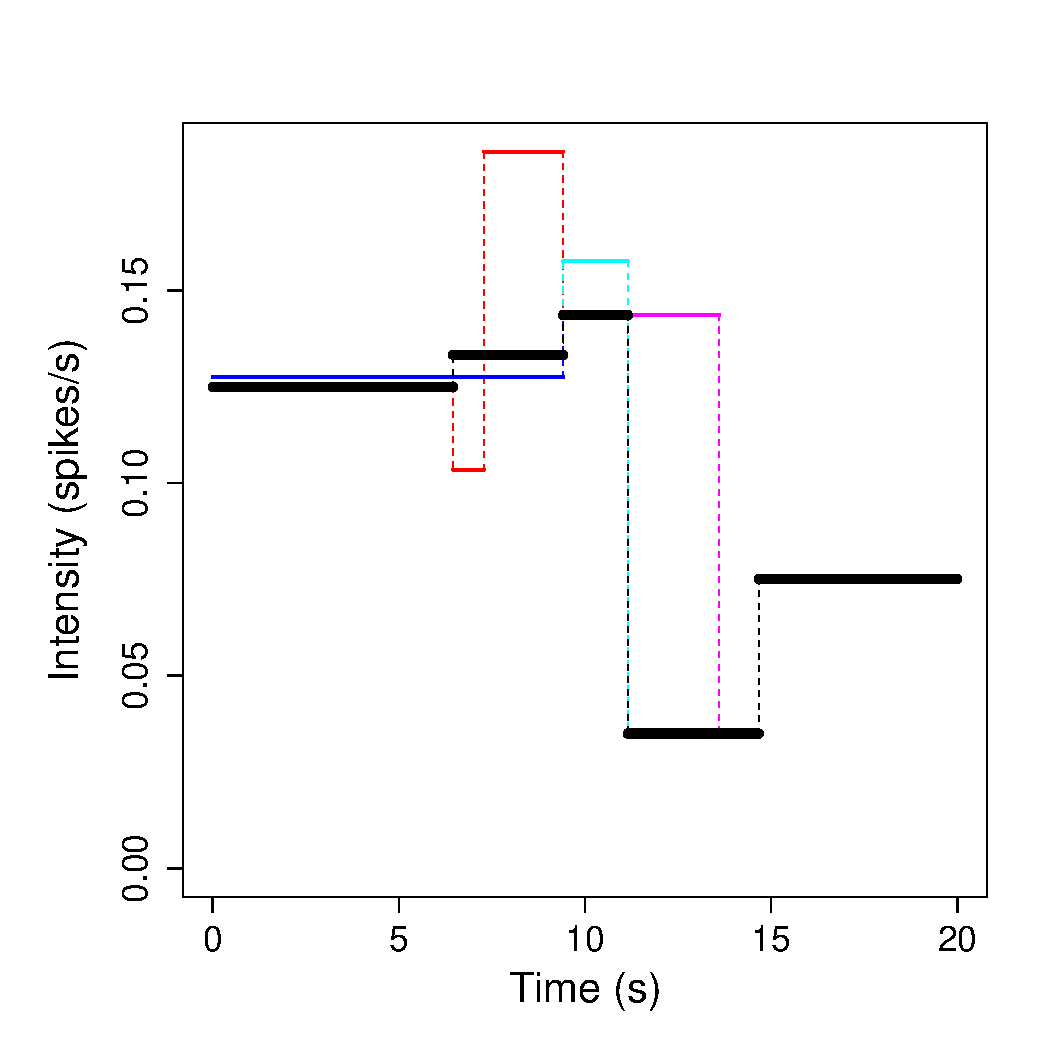
\includegraphics[scale = 0.4]{StepExample} }}
    \end{center}     
    \caption{Illustration of the possible moves at each iteration of the RJMCMC. The black line corresponds to the original step function. The blue line shows a candidate function when a change point is removed. Red when a new change point is added. Cyan when a height is changed. Magenta when a change point moves.  }
    \label{fig:PWCMove}
    \hrulefill
    \end{figure}

    %Birth
    \subsubsection{Step 1. Birth of a change point}
Firstly, we want to describe how to calculate the position of the new change point and how this changes the heights. Assume initially we have change points $s_1, \dots, s_k$ and corresponding heights $h_0, \dots, h_k$.  A new change point $s^*$ is chosen uniformly on $[0,T]$. The new change point lies in an existing interval $[s_j,s_{j+1})$ with probability 1.  So our set of change points becomes $\{s_1 , \dots, s_j, s^*, s_{j+1}, \dots, s_k \}$. 

%proposal
%Add that we use geometric
Next we want to propose the new heights. We will replace height $h_j$ (this corresponds to the interval $[s_j,s_{j+1})$ ) with two new heights $h'_j$ and $h'_{j+1}$, using a weighted geometric mean so that

\begin{equation}\label{eq:propose1}
(s^* - s_j) \log (h'_j) + (s_{j+1} - s^*) \log (h'_{j+1}) = (s_{j+1} - s_j ) \log (h_j)
\end{equation}

and
\begin{equation} \label{eq:propose2}
\frac{h'_{j+1}}{h'_j} = \frac{1-u}{u}
\end{equation}
where $u \sim \mathrm{U}(0,1)$. Hence the candidate heights are $h_0$, $\dots, h_{j-1}$, $h'_j, h'_{j+1}$, $h_{j+1}, \dots, h_k$.\\

The acceptance probability takes the form
\begin{multline}
p_{\mathrm{acc}} = \min \{1, \text{(likelihood ratio)} \times \text{(prior ratio)} \\  \times \text{(proposal ratio)} \times \text{(Jacobian)} \}.
\end{multline}

The likelihood and prior terms correspond to the target distribution, the proposal ratio is analogous to the transition ratio in the Metropolis-Hastings algorithm \eqref{eq:MH}, and the Jacobian is the transformation of coordinates from the original to the new space, e.g from $k$ changepoints to $k+1$. 

%prior ratio
Begin by deriving the prior ratio. In words we have:
\begin{multline}
\text{(prior ratio)} = \text{(prior ratio for heights)} \\ \times \text{(prior ratio for change points)}.
\end{multline}

Consider the heights. We assumed that the heights come from independent $\Gamma (\kappa, \mu)$ distributions. Thus, the probability of heights $h_0, \dots, h_k$ is

\begin{equation}
p(h_0, \dots, h_k) = \prod^k_{j=0} \frac{\mu^\kappa}{\Gamma (\kappa)} h_j^{\kappa-1}e^{-\mu h_j}. 
\end{equation}

Consequently, the ratio takes the form $ p(h_0, \dots, h'_j,h'_{j+1} , \dots, h_k)$ / $ p(h_0$, $\dots,$ $h_j $, $\dots, h_k) $, notice that all heights apart from $h_j, h'_j$ and $h'_{j+1}$ cancel in the division. Hence, the ratio reduces to $p(h'_j , h'_{j+1}) / p(h_j)$. Solving this gives:

\begin{align}
\text{(prior ratio for heights)} & =  \frac{\bigg( \big( \frac{\mu^\kappa}{\Gamma (\kappa)} \big)^2 (h'_j)^{\kappa-1} e^{-\mu h'_j} (h'_{j+1})^{\kappa-1}e^{-\mu h'_{j+1}} \bigg)}
{\bigg(\frac{\mu^\kappa}{\Gamma (\kappa)} h_j^{\kappa-1} e^{-\mu h_j}   \bigg)}, \\
& =  \frac{\mu^\kappa}{\Gamma (\kappa)} \bigg(\frac{h'_j h'_{j+1}}{h_j}\bigg)^{\kappa-1} \exp \{- \mu (h'_j + h'_{j+1} - h_j) \}.  \label{eq:ratioH}
\end{align}

Next consider the change points. Each individual change point is uniformly distributed on $[0,T]$, i.e $s_i \sim U[0,T]$, with density $p(s_i) = 1/T$ for $i = 1, \dots, k$. Hence considering the joint distribution we get
%We assume that the change points are distributed as the even numbered order statistics of $2k+1$ points uniformly and independently distributed on $[0,T]$. 
%The probability of $s_1 , \dots , s_k$ is 
%\begin{equation}\label{eq:cp}
%p(s_1, \dots, s_k) = \frac{(2k+1)!}{T^{2k+1}} (s_2-s_1) \dots (s_{j+1}-s_j) \dots (s_{k+1}-s_{k}).
%\end{equation}


\begin{align}
p(s_1, \dots, s_k) &= (2k+1)!\int \dots \int \frac{1}{T^{2k+1}} \mathbbm{1}_{ \left\{ s_0 < t_1 <s_1 < t_3 < s_2 < t_5 \dots \right\}} dt_1 dt_3 \dots dt_{2k+1}, \\
&= \frac{(2k+1)!}{T^{2k+1}}\int \dots \int \mathbbm{1}_{ \left\{ s_0 < t_1 <s_1 < t_3 < s_2 < t_5 \dots \right\} } dt_1dt_3 \dots dt_{2k+1},  \\
&= \frac{(2k+1)!}{T^{2k+1}} (s_1-s_0) \dots (s_{j+1}-s_j) \dots (s_{k+1}-s_{k}),\label{eq:cp}
\end{align}

where $s_0 = 0$ and $s_{k+1} = T$, are the start and end times of the experiment. Furthermore, $(2k+1)!$ comes from the number of permutations of $2k+1$ points. Hence the prior probability of having $k$ change points at times $\{s_i \}_{i=1}^k$ is $\eqref{eq:Poiss} \times \eqref{eq:cp}$, where we leave the conditioned Poisson as $p(k)$ for simplicity in the following equations. Similar to the heights ratio, all the factors of the form $(s_{i+1} - s_i)$, $i=1, \dots, k$ cancel except for the intervals that have been changed by the introduction of the new point $s^*$. 
Thus giving

\begin{align}
\text{(prior ratio for change points)} & = \frac{\bigg( p(k+1)\frac{(2k+3)!}{T^{2k+3}} (s^* - s_j) (s_{j+1} - s^*) \bigg) }
{ \bigg(  p(k)\frac{(2k+1)!}{T^{2k+1}} (s_{j+1} - s_j)\bigg)},  \\
& = \frac{p(k+1)}{p(k)} \frac{(2k+2)(2k+3)}{T^2} \frac{(s^* - s_j) (s_{j+1} - s^*) }{(s_{j+1} - s_j)}. \label{eq:ratioCP}
\end{align}

Putting together equation \eqref{eq:ratioH} and \eqref{eq:ratioCP} we get that the prior ratio is
\begin{multline}
\text{(Prior ratio)} = \frac{p(k+1)}{p(k)} \frac{(2k+2)(2k+3)}{T^2} \frac{(s^* - s_j) (s_{j+1} - s^*) }{(s_{j+1} - s_j)}  
 \\ \times \frac{\mu^\kappa}{\Gamma (\kappa)} \bigg(\frac{h'_j h'_{j+1}}{h_j}\bigg)^{\kappa-1}  \exp \{- \mu (h'_j + h'_{j+1} - h_j) \}. 
\end{multline}\\
%proposal ratio
%Need to explain what x is.
Next we want to compute the proposal ratio. As stated previously, this is analogous to the ratio $q(x'|x) / q(x|x')$, where $x$ is the current value of the intensity function and $x'$ the candidate value. In this case where we are now jumping between different dimensions this becomes $j(x') / (j(x) q(u) )$, where $j(x)$ is the probability of choosing $x$ and q(u) is the choice of the parameter $u$ used to generate the new point in the space. Hence, $j(x')$ is the move from $x'$ to $x$ which is a death at the point $s^*$ and $j(x)$ is the move from $x$ to $x'$ which is the birth of point $s^*$.
\begin{equation}
\text{(Proposal Ratio)} = \frac{j(x')}{j(x)q(u)} = \frac{d_{k+1} \frac{1}{k+1}}{b_k \frac{1}{T - 0}\frac{1}{1-0}} = \frac{d_{k+1}T}{b_k (k+1)}.
\end{equation} 
%jacobian
The Jacobian calculates the change in co-ordinates from our original space to the candidate space. Due to the nature of adding a single change point this reduces to the change from $h_j$ (and $u$) to $h'_j$ and $h'_{j+1}$. We first need to rearrange equations \eqref{eq:propose1} and \eqref{eq:propose2}   to $h'_j$ and $h'_{j+1}$ in terms of $h_j$ and $u$. This is done initially taking the exponential
\begin{equation}
\left( h'_j \right) ^{ \left(s^* - s_j \right)} \left( h' _{j+1} \right)^{ \left(s_{j+1} - s^* \right)} = h_j^{\left( s_{j+1} - s_j  \right)}.
\end{equation}
Then we substitute $h'_{j+1} = h'_j\frac{1-u}{u}$, thus getting the exponent for $h'_j$ to be $\left( s_{j+1} - s_{j} \right) $. Hence, rearranging for $h'_j$ we get
 \begin{equation}
h'_j = h_j \left( \frac{u}{1-u}\right) ^{\frac{s_{j+1} -s^*}{s_{j+1} - s_j}}.
\end{equation} 
Similarly, for $h'_{j+1}$ we have
\begin{equation}
h'_{j+1} = h_j \left( \frac{1-u}{u}\right) ^{\frac{s^*-s_j}{s_{j+1} - s_j}}.
\end{equation} 
  For ease of notation we let $r = (s_{j+1} - s^*) / (s_{j+1} - s_j)$, and ergo $1-r = (s^* - s_j) / (s_{j+1} - s_j) $ from now on. 
%Need explaination of why the jacobian reduces to just the determinant of the 2x2.

\begin{align}
J &= 
\begin{vmatrix}
\frac{\partial h'_j}{\partial h_j} & \frac{\partial h'_j}{\partial u} \\
\frac{\partial h'_{j+1}}{\partial h_j} & \frac{\partial h'_{j+1}}{\partial u} 
\end{vmatrix}, \\
&= \begin{vmatrix}
\big(\frac{u}{1-u}\big)^r & h_j r \big(\frac{u}{1-u}\big)^{r-1} \frac{1}{(1-u)^2} \\
\big(\frac{1-u}{u}\big)^{1-r} & h_j (1-r) \big(\frac{1-u}{u}\big)^{-r} \frac{-1}{u^2}
\end{vmatrix}, \\
&= h_j (1-r) \frac{u^{2r-2}}{(1-u)^{2r}} + h_j r \frac{u^{2r-2}}{(1-u)^{2r}}, \\
&= h_j \frac{u^{2r-2}}{(1-u)^{2r}}, \\
&= h_j \frac{ [u^{r-1} u + u^{r-1}(1-u)]^2}{(1-u)^{2r}}, \\
&= \frac{[h_j (\frac{u}{1-u})^r + h_j (\frac{1-u}{u})^{1-r} ]^2}{h_j}, \\
&= \frac{(h'_j + h'_{j+1})^2}{h_j}.
\end{align}  


    %death
    \subsubsection{Step 2. Death of a change point}
 Select a change point $s_{j+1}$ uniformly at random from the existing change points for deletion, and propose new height $h'_j$ over the interval $(s_{j},s_{j+2}) = (s'_j,s'_{j+1})$ by
 
 \begin{equation}
 (s_{j+1} - s_j) \log(h_j) + (s_{j+2} - s_{j+1}) \log (h_{j+1} ) = (s'_{j+1} - s'_j) \log(h'_j) .
 \end{equation} 

The acceptance probability is obtained by inversion of the terms for the corresponding birth probability. Hence the prior ratio is

\begin{multline}
\frac{p(k-1)} {p(k)}\frac{T^2}{2k(2k+1)} \frac{(s'_{j+1} - s'_j)}  {(s_{j+2} - s_{j+1}) (s_{j+1} - s_j) }
 \\ \times \frac{\Gamma (\kappa)}{\mu^\kappa} \bigg(\frac{h'_j}{h_j h_{j+1}}\bigg)^{\kappa-1} \exp \{- \mu (h'_j  - h_j - h_{j+1}) \}, 
\end{multline}

the proposal ratio is


\begin{equation}
 \frac{b_{k-1} k}{d_{k}T},
\end{equation} 

and the Jacobian is

\begin{equation}
\frac{h'_j}{(h_j + h_{j+1})^2} .
\end{equation} 

%Within model change
    \subsubsection{Step 3. Within model updates}
When we are not proposing a birth or a death, the following within model updates take place.\\

Move an existing change point: provided that $k>0$ a change point $s_j$ is chosen uniformly at random from the existing change points and a new position $s'_j$ is proposed uniformly at random on $[s_{j-1}, s_{j+1}]$ and accepted with probability

 \begin{equation} \label{eq:WithinCP}
\min \bigg\{1, \text{(likelihood ratio)} \times \frac{(s_{j+1} - s'_j)(s'_j - s_{j-1})}{(s_{j+1} - s_j)(s_j - s_{j-1})} \bigg\}
\end{equation}  \\

Change a height: a height $h_j$ is chosen uniformly at random from the existing heights and a new height $h'_j$ is proposed such that $\log(h'_j/h_j)$ is uniformly distributed on $[-1/2,1/2]$, and accepted with probability

 \begin{equation}\label{eq:WithinH}
\min \big\{1, \text{(likelihood ratio)} \times (h'_j/h_j)^\kappa \exp \{ -\mu(h'_j - h_j) \} \big\}
\end{equation}  \\

The second term in equations \eqref{eq:WithinCP} and \eqref{eq:WithinH} come from the prior distribution for the change points and heights respectively. \\

In the steps above we have used the assumption that the heights are a priori independent and identically distributed. We will now discuss how the calculations change with the martingale structure. This change  does not affect the mechanism of which move is used in an iteration nor how we propose the candidate function. Changes only occur via the prior ratio in the acceptance probability. 

First, consider a birth of a new point. Recall that the original heights are $h_0, \dots h_k$ and the proposed heights are $h_0, \dots, h_{j-1}, h'_j, h'_{j+1}, h_{j+1}, \dots, h_k$ and the only change comes from replacing height $h_j$ with heights $h'_j$ and $h'_{j+1}$, where for the martingale structure we have $h_i \sim \Gamma(\kappa, \frac{\kappa}{h_{i-1}})$, for $i>0$ and $h_0 \sim \Gamma(\kappa,\mu)$.  Notice that even with the more complex structure most of the terms will cancel in the prior ratio. In fact, the probability of each height only depends on the previous height, thus the ratio simplfies to $p(h'_{j}, h'_{j+1},h_{j+1})/p(h_j,h_{j+1}) $. We will need to spilt into 2 cases, for when $j<k$ and $j=k$ since $h_{j+1}$ does not exist if $j=k$. Furthermore, care needs to be taken when only one height exists, as the ratio simplifies further to $p(h'_{1}, h'_{2})/p(h_1)$.

First lets consider the simpler case when $j=k$, explicitly writing the prior ratio gives the following 
\begin{equation}
\frac{\left( \frac{\left(\kappa /h_{k-1}\right)^\kappa}{\Gamma \left( \kappa \right)} \left( h'_k \right)^{\kappa-1} \exp \left\{ -\frac{\kappa}{h_{k-1}}h'_k \right\}     \right) 
\left( \frac{\left(\kappa /h'_{k}\right)^\kappa}{\Gamma \left( \kappa \right)} \left( h'_{k+1} \right)^{\kappa-1} \exp \left\{ -\frac{\kappa}{h'_{k}}h'_{k+1} \right\}     \right)}
{\left( \frac{\left(\kappa /h_{k-1}\right)^\kappa}{\Gamma \left( \kappa \right)}  h_k ^{\kappa-1} \exp \left\{ -\frac{\kappa}{h_{k-1}}h_k \right\}     \right)}
\end{equation}
 Then collecting terms and simplifying gives \begin{equation}
\text{(Prior ratio)} = \frac{\kappa^\kappa}{\Gamma \left( \kappa \right)} \frac{1}{h_k} \left(\frac{h'_{k+1}}{h'_k}\right)^{\kappa-1} \exp \left\{ \kappa \left( \frac{h_k -h'_k}{h_{k-1}} - \frac{h'_{k+1}}{h'_k}  \right) \right\}
\end{equation}

Now consider the case where $j<k$, for simplicity define $h_{-1} = \mu$  because $h_0 \sim \Gamma (\kappa, \mu)$. 

\begin{equation}
\dfrac{\splitdfrac{\left( \frac{\left(\kappa /h_{j-1}\right)^\kappa}{\Gamma \left( \kappa \right)} \left( h'_j \right)^{\kappa-1} \exp \left\{ -\frac{\kappa}{h_{j-1}}h'_j \right\}     \right) 
\left( \frac{\left(\kappa /h'_{j}\right)^\kappa}{\Gamma \left( \kappa \right)} \left( h'_{j+1} \right)^{\kappa-1} \exp \left\{ -\frac{\kappa}{h'_{j}}h'_{j+1} \right\}     \right)  }{
\times \left( \frac{\left(\kappa /h'_{j+1}\right)^\kappa}{\Gamma \left( \kappa \right)} \left( h_{j+1} \right)^{\kappa-1} \exp \left\{ -\frac{\kappa}{h'_{j+1}}h_{j+1} \right\}     \right)}}
{\left( \frac{\left(\kappa /h_{j-1}\right)^\kappa}{\Gamma \left( \kappa \right)} \left( h_j \right)^{\kappa-1} \exp \left\{ -\frac{\kappa}{h_{j-1}}h_j \right\}     \right)
\left( \frac{\left(\kappa /h_{j}\right)^\kappa}{\Gamma \left( \kappa \right)} \left( h_{j+1} \right)^{\kappa-1} \exp \left\{ -\frac{\kappa}{h_{j}}h_{j+1} \right\}     \right)}
\end{equation}

Simplifying 
\begin{equation}
\frac{\kappa^\kappa}{\Gamma \left( \kappa \right)} \frac{h_j}{h'_j + h'_{j+1}} \exp \left\{ \kappa \left( -\frac{h'_j - h_j}{h_{j-1}} - \frac{h'_{j+1}}{h'_j} - \frac{h_{j+1}}{h'_{j+1}} 
+\frac{h_{j+1}}{h_j} \right)   \right\}
\end{equation}


Similar to before, for a death of a change point we just inverse the prior for the birth. There is no affect for changing the value of a change point. Next consider changing a height, again we must split into two cases when $j<k$ and $j=k$ repeating the argument above we get the prior ratio to be 

%If j=k then for the prior we have 
%\begin{equation}
%\frac{\left( \frac{\left(\kappa /h_{k-1}\right)^\kappa}{\Gamma \left( \kappa \right)} \left( h'_k \right)^{\kappa-1} \exp \left\{ -\frac{\kappa}{h_{k-1}}h'_k \right\}     \right)}
%{\left( \frac{\left(\kappa /h_{k-1}\right)^\kappa}{\Gamma \left( \kappa \right)}  h_k ^{\kappa-1} \exp \left\{ -\frac{\kappa}{h_{k-1}}h_k \right\}     \right)}
%\end{equation}
%
% simplifying 
 
 \begin{equation}
\left( \frac{h'_j}{h_j} \right )^{\kappa-1} \exp \left\{ - \frac{\kappa}{h_{j-1}} \left( h'_j - h_j \right) \right\},
\end{equation}

for $j=k$, and
 
%If $j < k$ then 
%\begin{equation}
%\frac{\left( \frac{\left(\kappa /h_{j-1}\right)^\kappa}{\Gamma \left( \kappa \right)} \left( h'_j \right)^{\kappa-1} \exp \left\{ -\frac{\kappa}{h_{j-1}}h'_j \right\}     \right)
%\left( \frac{\left(\kappa /h'_{j}\right)^\kappa}{\Gamma \left( \kappa \right)} \left( h_{j+1} \right)^{\kappa-1} \exp \left\{ -\frac{\kappa}{h'_{j}}h_{j+1} \right\}     \right)}
%{\left( \frac{\left(\kappa /h_{j-1}\right)^\kappa}{\Gamma \left( \kappa \right)}  h_j ^{\kappa-1} \exp \left\{ -\frac{\kappa}{h_{j-1}}h_j \right\}     \right)
%\left( \frac{\left(\kappa /h_{j}\right)^\kappa}{\Gamma \left( \kappa \right)} \left( h_{j+1} \right)^{\kappa-1} \exp \left\{ -\frac{\kappa}{h_{j}}h_{j+1} \right\}     \right)}
%\end{equation}
%
%simplifying
 \begin{equation}
 \frac{h_j}{h'_j}  \exp \left\{ -\frac{\kappa}{h_{j-1}} \left(h'_j - h_j \right) - \kappa h_{j+1} \left( \frac{1}{h'_j} - \frac{1}{h_j} \right)\right\},
\end{equation}

for $j<k$. This replaces $ (h'_j/h_j)^\kappa \exp \{ -\mu(h'_j - h_j)$ in \eqref{eq:WithinH}.


%%%%%%%%%%%%%%%%%%%%%%%%%%%
%% Gaussian Process Model
%%%%%%%%%%%%%%%%%%%%%%%%%%%
\subsection{Gaussian Process Prior}
%Figure of Gaussian Process
  \begin{figure}[t]
   \hrulefill
   \begin{center} 
    \subfloat{{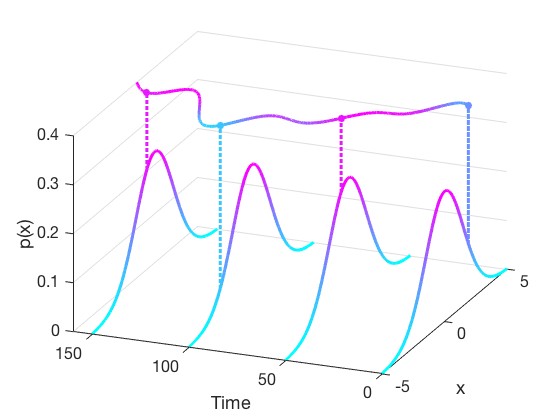
\includegraphics[scale = 0.4]{BasicGP} }}
    \end{center}     
    \caption{Realisation of a Gaussian Process (top line), with mean 0 and SE covariance. The bell shape curves show the probability distributions of the values the realisation can take at times 0, 50, 100 and 150, where the probability is coloured such that light blue indicates low probability and magenta high probability. The dashed lines indicated the probability of the given value that the GP takes at that time.   }
    \hrulefill
    \label{fig:BasicGP}
    \end{figure}
    
A Gaussian process (GP) is a collection of random variables where any finite number of which have a multivariate Gaussian distribution. A GP is fully specified by its mean and covariance function. Often the mean is taken to be 0, in which case a GP is defined solely by its covariance function.  There are many potential covariance functions that could be used such as: constant, linear, or Gaussian noise \cite{rasmussen2004}. However, we use the widely applied standard squared exponential (SE) covariance function, 
\begin{equation}\label{eq:Cov}
\Sigma(t_1,t_2) = \sigma_f^2 \exp \bigg[ \frac{(t_1 - t_2)^2}{2l^2} \bigg] + \delta (t_1 - t_2) \sigma_v^2.
\end{equation}
    This is because realisations from the GP with SE covariance are smooth when $\sigma_v^2 = 0$, which is a property we desire for the intensity function, to mimic the varying stimulus that cells experience in vitro. Three hyper parameters define the shape of the intensity function, as can be seen in figure \ref{fig:GPVary}.
         %Figure of varying GP parameters
  \begin{figure}[h]
   \hrulefill
   \begin{center} 
    \subfloat[]{{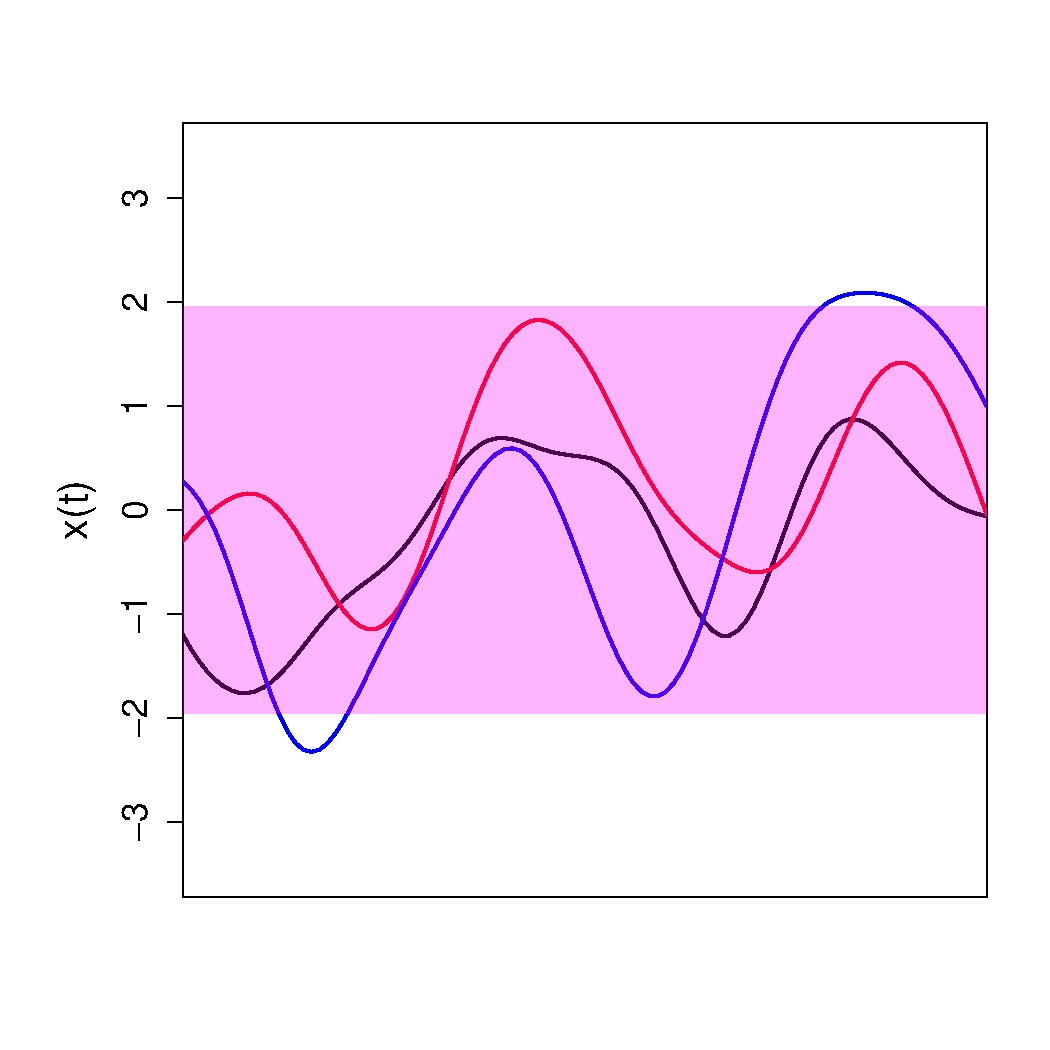
\includegraphics[scale = 0.35]{GP_vary1} }} \quad
      \subfloat[]{{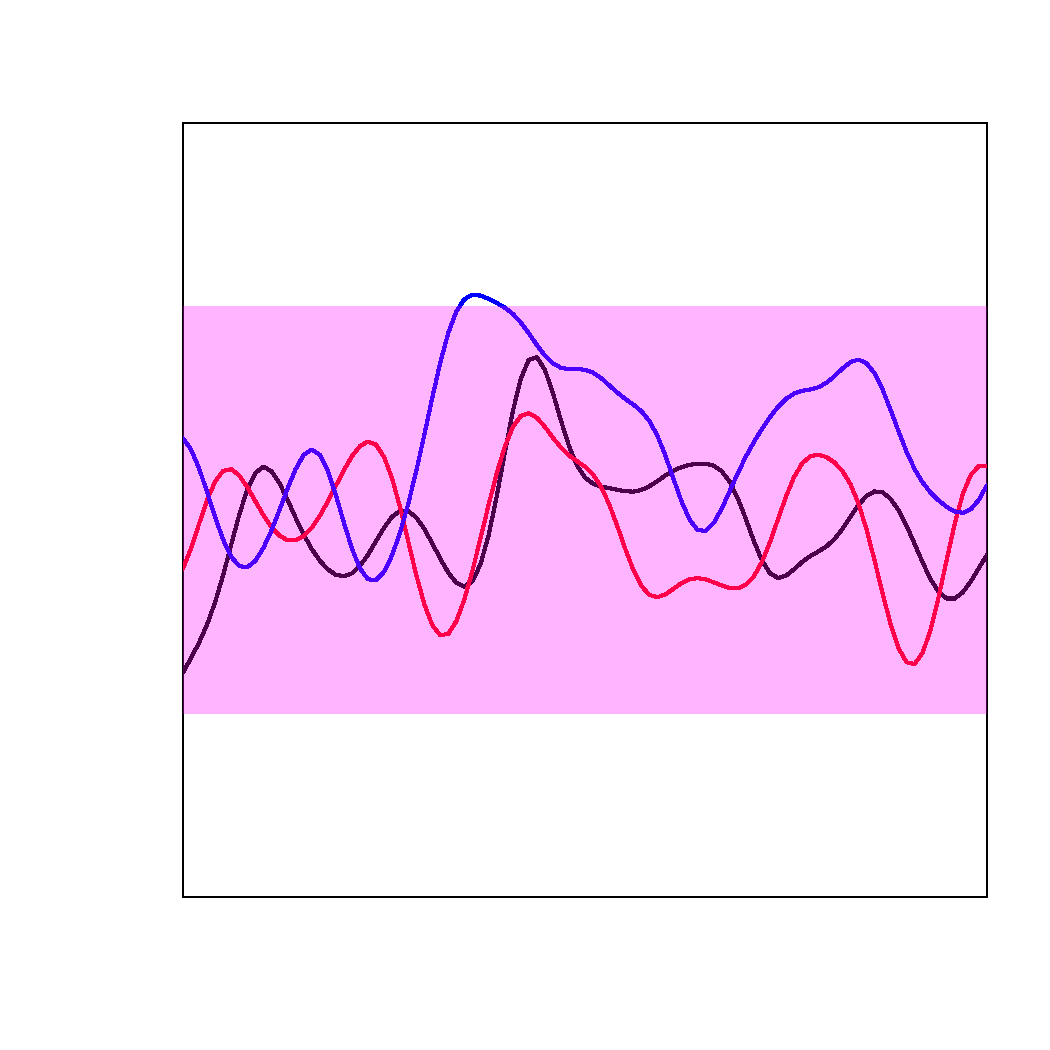
\includegraphics[scale = 0.35]{GP_vary2} }} \vspace{0.1mm} 
  \subfloat[]{{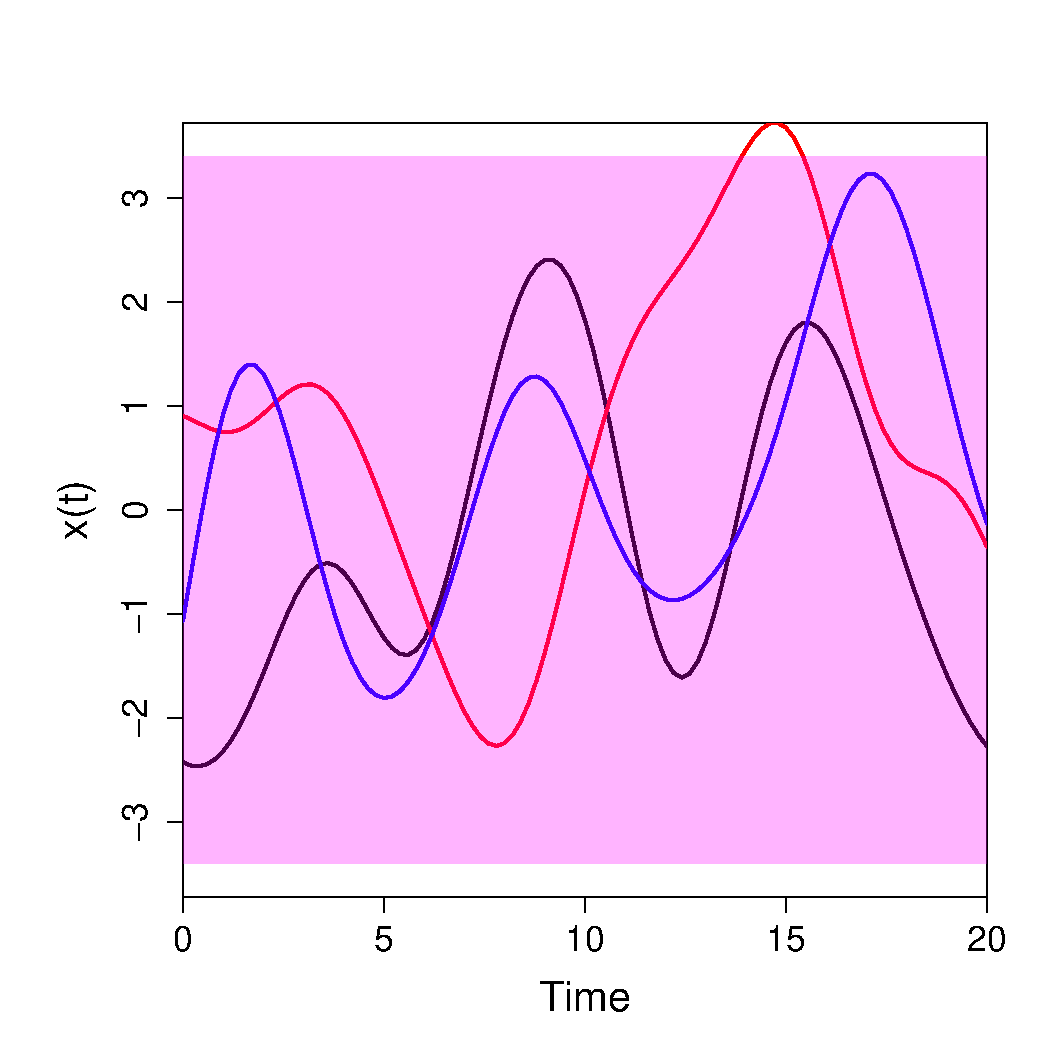
\includegraphics[scale = 0.35]{GP_vary3} }} \quad
  \subfloat[]{{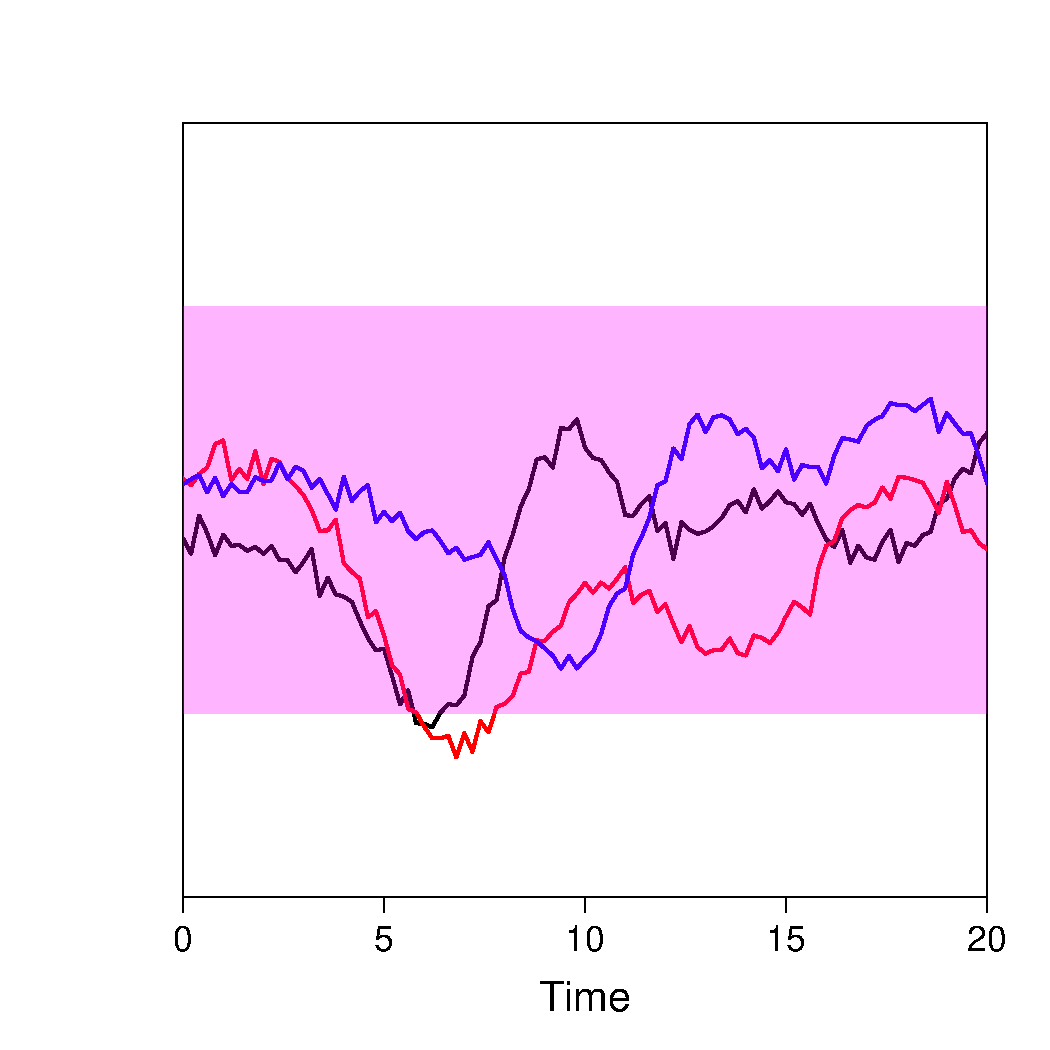
\includegraphics[scale = 0.35]{GP_vary4} }} 
    \end{center}     
    \caption{Illustration of how varying hyper parameters changes realisations of a Gaussian Process with mean 0. We draw 3 samples from the following GP priors: (A) $\sigma_f^2 = 1, l = 2, \sigma_v^2 = 0 $ (B) $\sigma_f^2 = 1, l = 1, \sigma_v^2 = 0 $ (C) $\sigma_f^2 = 2, l = 2, \sigma_v^2 = 0 $ (D) $\sigma_f^2 = 1, l = 2, \sigma_v^2 = 0.01.$ The magenta region indicates the 95\% confidence intervals. In (B) we notice that decreasing the length scale leads the realisation to vary more frequently with time. In (C) increasing $\sigma^2_f$ increases the range of values taken (variance). Finally, (D) shows noise is controlled by $\sigma^2_v$.     }
    \label{fig:GPVary}
    \hrulefill
    \end{figure}%Or by definition 
      $\sigma_f^2$ determines the function's average distance from the mean (fig \ref{fig:GPVary}A, \ref{fig:GPVary}C); $l$ controls the `smoothness' of the intensity, where smaller $l$  leads to an intensity that varies more (fig \ref{fig:GPVary}A, \ref{fig:GPVary}B) and $\sigma_v^2$ is additional Gaussian noise (fig \ref{fig:GPVary}A, \ref{fig:GPVary}D). 
 

    
    A Gaussian process can be viewed as a probability distribution over the space of functions on $[0,T]$, the domain of interest. For example in figure \ref{fig:BasicGP} the top line is a draw from the GP with mean 0 and SE covariance function, each curve underneath corresponds to the normal distribution that that point comes from, where magenta corresponds to a higher probability of the value occurring and blue a lower probability.  
     
     To sample from a GP we discretise time by partitioning the interval into $\mathbf{t} = \{t_i \}^M_{i=1} $, where $t_i = i \Delta$ such that $\Delta$ is the time step used. From these points we can retrieve the covariance matrix $\mathbf{\Sigma} = \left\{ \Sigma (t_i, t_j ) \right\}_{t_i , t_j  \in \mathbf{t}}$, assuming the GP has mean $\mu$, a vector of length M,  we can approximate a realsiation from the GP by sampling from the multivariate normal with mean $\mu$ and covariance matrix $\mathbf{\Sigma}$. 
     
     Furthermore, we can calculate the probability of a function $f(t)$ by discretising to $\mathbf{f} = \{f_i \}^M_{i=1}$ with $f_i = f(t_i)$ and evaluating the probability density function for the Multivariate normal distribution, i.e $ \mathcal{N}(\mathbf{f} | \mathbf{ \mu}, \mathbf{\Sigma})$. 
    Next we consider how to use a GP as a prior for our intensity function $x(t)$, as noted above we need to discretise the intensity function for practical purposes, thus $x(t)$ becomes $\mathbf{x} = \{ x_i\}^M_{i=1}  $, where $x_i = x(t_i)$. Often the time step $\Delta$ is taken to be the inverse of the recording frame rate of the experiment such that spikes occur on the discretised grid.  However, care needs to be taken if the spike data is altered before fitting the model, such as removing linear trends. In this situation, the altered spike times do not occur on  the grid created from the experiment frame rate. To combat this, we extend the grid to include the spike times, for example if the original grid is $\mathbf{t} = \{t_i \}^M_{i=1} $, we extend to $\mathbf{\tilde t} = \mathbf{t} \cup \mathbf{y}$, where $\mathbf{y}$ are the spike times.
    
    For the Gamma ISI distribution we obtain the likelihood function with the discretisation to be
\begin{equation}
\pi (\mathbf{y} | \mathbf{x}, \gamma) = x_{1} e^{-\hat X_{0,1}} e^{-\hat X_{n, n+1}} \prod^{N}_{i=2} \frac{ \gamma x_{l_i}}{\Gamma (\gamma )} \left[ \gamma \hat X_{i-1,i} \right] ^{\gamma -1} e^{-\gamma \hat X_{i-1,i}},
\end{equation}   
where $\hat X_{i,j} = \Delta \sum^{l_j}_{k = l_i} x_k$ with $l_0 = 0$, and $l_{n+1} = T/ \Delta$. Since we are only considering updating $x$ we can remove terms purely in $\gamma$, to get 
\begin{equation}\label{eq:xlikeli}
\pi (\mathbf{y} | \mathbf{x},\gamma) = x_{1} e^{-\hat X_{0,1}} e^{-\hat X_{n, n+1}} \prod^{N}_{i=2} x_{l_i} \left[\hat X_{i-1,i} \right] ^{\gamma -1} e^{-\gamma \hat X_{i-1,i}} .
\end{equation}    

Note that we require the intensity function to be positive, as it is impossible to have a negative spiking rate. 
Thereby, we will assume that the logarithm of the intensity function has a Gaussian Process prior with SE covariance, that is 
\begin{equation}\label{eq:prior}
\log \mathbf{x} \sim \mathcal{N} ( \mathbf{0} , \mathbf{\Sigma}  ),
\end{equation}

where $\mathbf{\Sigma}$ is defined in \eqref{eq:Cov}.

It is not necessary to take the logarithm, however when sampling the posterior distribution of $x(t)$ many proposed intensity functions would not be positive and would be rejected instantaneously, requiring a longer mixing time.  

Hence in general, with the GP prior the unknowns are the model parameters and the hyper parameters of the GP, i.e $\{x, \theta, \sigma_f^2, l, \sigma_n^2 \}$. However, we elect to fix $\sigma_f^2 = 1000$ to allow for a large range of intensity values, equivalent to adding a non-informative prior about the value of the intensity. To determine realisations from the GP we need to be able to sample from a large multivariate normal distribution which requires inversion of the covariance matrix. We want to set $\sigma_n^2 = 0$ to retain the smoothness property of the intensity function, however doing such renders the matrix computationally singular. Hence, we set  $\sigma_n^2  = 0.0001$, small, hereby making the inversion possible with negligible random noise. This is equivalent to adding a nugget term to the Gaussian process \cite{Nugget}.  A priori we have little information to inform us on a sensible value for $l$. For this reason we keep it as a model parameter. Thus for the GP prior we introduce a new variable $l$ which we also need to predict.  As $\mathbf{x}$ requires a complex MCMC algorithm we sample $l$ separately from $x$, utilising Gibbs Method.

%%%%%%%%%%%%%%%%%%%ALGOR%%%%%%%%%%%%%%%%%%%%%%%%%%%%%%%
\begin{algorithm}[t]
\DontPrintSemicolon
\textbf{Input:} \text{$\mathbf{y}$, ISI distribution,  $T$, $M$, $M_\mathrm{burn}$, $\mathbf{t}$, $\omega,\sigma^2_\theta, \sigma^2_l$ } \\
\textbf{Output:} \text{M samples of intensity $\mathbf{x}$, ISI parameter $\theta$ and length } \\ \text{scale $l$.} \\
Set initial values $\mathbf{x}^{(0)}, \theta^{(0)}$ and $l^{(0)}$; \; 
\For{$i$ in $1$ to ($M+M_\mathrm{burn}$)}{
\textbf{Step 1.} Propose $\mathbf{x}_{\mathrm{can}}$ and calculate acceptance probability using underrelaxed method, update $\mathbf{x}^{(i)}$; \;
\textbf{Step 2.}Propose $l_{\mathrm{can}}$  and calculate acceptance probability using RW-Metropolis, update $l^{(i)}$; \;
\textbf{Step 3.}Update $\theta_{\mathrm{can}}$and calculate acceptance probability using RW-Metropolis, update $\theta^{(i)}$ (section 1.4.4); \; 
}
\text{Return:} $\mathbf{x}, \theta$ and $l$ with initial $M_\mathrm{burn}$ iterations removed; 
\caption{Inference for GP prior.}
\end{algorithm}

In algorithm 3 we give an outline of the method used, where the required inputs are: the spikes $\mathbf{y}$; the ISI distribution used (e.g. Gamma, Weibull, etc); the experiment length $T$; the number of samples we need $M$ and the initial number of iterations to remove $M_\mathrm{burn}$; the discretisation $\mathbf{t}$ used for the GP; step-size parameter $\omega$ used in the under-relaxed method and the variances $\sigma^2_\theta, \sigma^2_l$ used in the RW-Metropolis algorithms for $\theta$ and $l$ respectively..  

In the upcoming sections we describe in detail the under-relaxed method used to update $\mathbf{x}$, followed by the RW-Metropolis algorithm used for $l$. 

%Figure of How to move in GP.
  \begin{figure}[t]
   \hrulefill
   \begin{center} 
    \subfloat{{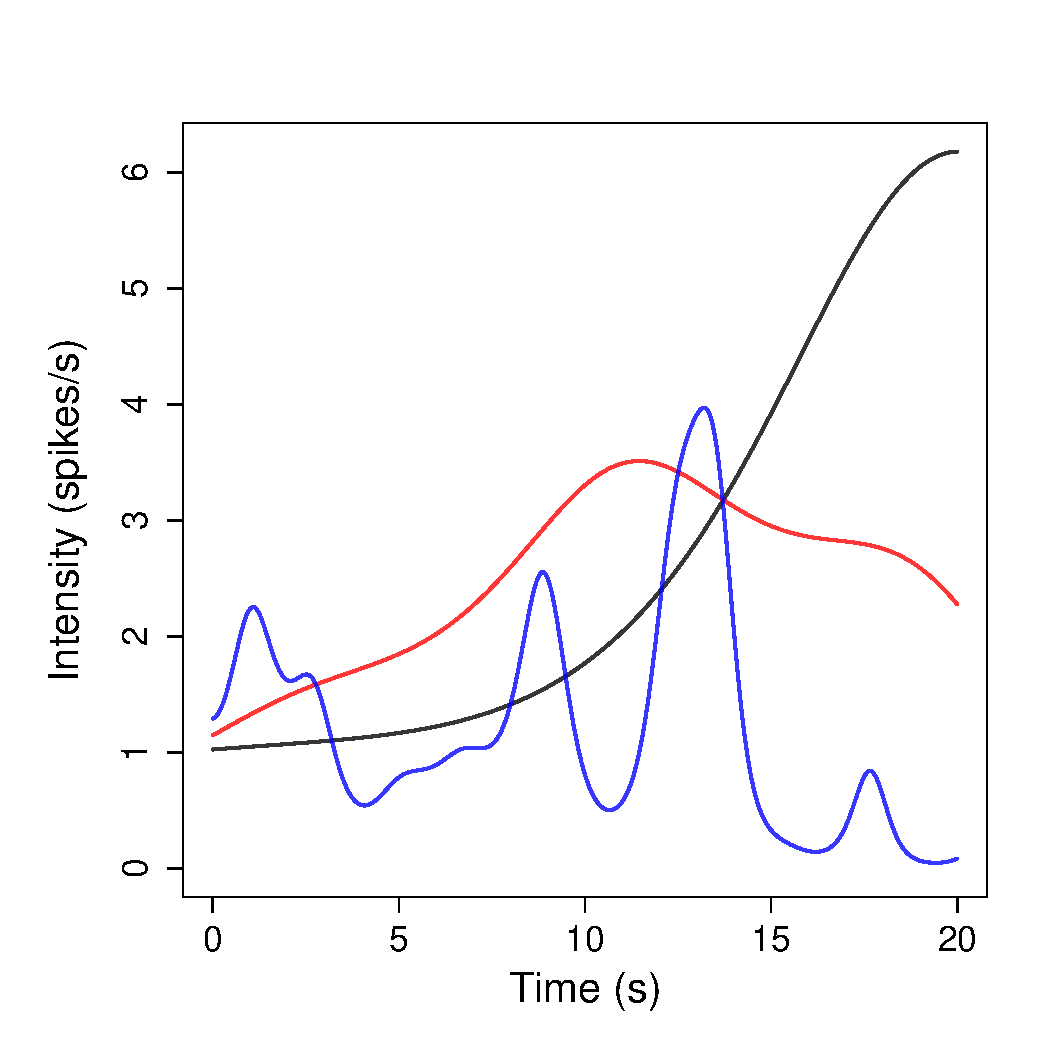
\includegraphics[scale = 0.4]{Draw_GP} }}
    \end{center}     
    \caption{Draws from the GP prior for the intensity, where we assume the logarithm of $x(t)$ has a GP prior. Where the black, red and blue lines correspond to length scales 10, 5 and 1. To illustrate that a priori we don't know the value of $l$ and it will be fitted using MCMC. }
    \label{fig:DrawGP}
    \hrulefill
    \end{figure}


% Posterior Calculation. 
\subsubsection{Step 1. Posterior Computation for $\mathbf{x}$}

We use a under-relaxed algorithm, based on a Metropolis-Hastings method \cite{NEAL}. Begin by choosing an initial value $\mathbf{x}_0$. As $x(t)$ describes the spiking rate, we set $\mathbf{x}_0$ to be the mean spike rate from the experiment. For example if an experiment ran for 100s and a total of 58 spikes were recorded then $\mathbf{x}_0 = \mathbf{0.58}$, the vector of length $M$ with all values equal 0.58. 
Consider an iteration, with current intensity $\mathbf{x}_{\mathrm{cur}}$, we propose new intensity $\mathbf{x}_{\mathrm{can}}$ by $\mathbf{x}_{\mathrm{can}} = e^{\mathbf{x}^*_{\mathrm{can}}}$ where

\begin{equation}\label{eq:GPpropose}
\mathbf{x}^*_{\mathrm{can}} = \sqrt{1-\omega^2} \log (\mathbf{x}_{\mathrm{cur}} ) + \omega \boldsymbol{\nu}, 
\qquad \qquad \boldsymbol{\nu} \sim \mathcal{N}(\mathbf{0}, \Sigma ).
\end{equation}

Above $\omega \in [-1,1] $ is a step-size parameter, where the closer $\omega$ is to zero the more the candidate value will be similar to the current value. Whereas, if $\omega$ is close to one the candidate value will be similar to a draw from the prior distribution. We use a value close to zero, often $\omega = 0.01$,  to improve the mixing of the MCMC (i.e candidate values get accepted more often).

Next we need to determine the acceptance probability, 
\begin{equation}\label{eq:GPacc}
p_{\mathrm{acc}} = \min \left\{ 1, \frac{\pi \left( \mathbf{y} | \mathbf{x}_{\mathrm{can}}, \theta \right) \pi\left(  \mathbf{x}_{\mathrm{can}}\right) q \left( \mathbf{x}_{\mathrm{cur}} |\mathbf{x}_{\mathrm{can}} \right)}
{\pi \left( \mathbf{y} | \mathbf{x}_{\mathrm{cur}}, \theta \right) \pi \left(  \mathbf{x}_{\mathrm{cur}} \right) q \left( \mathbf{x}_{\mathrm{can}} |\mathbf{x}_{\mathrm{cur}} \right)} \right\}
\end{equation}
where for the Gamma ISI distribution $\pi \left( \mathbf{y} | \mathbf{x},\theta \right)$ comes from \eqref{eq:xlikeli}, the prior $\pi (\mathbf{x})$ is defined in \eqref{eq:prior} and $q( r | s )$ is the probability of transitioning from intensity $s$ to $r$. Due to the proposal regime this reduces to only the marginals since the prior and $q$ ratios cancel out. % \footnote{See appendix A.}

% Text about the cancelation for the base case where x is a single variable and no log business.
For simplicity we show that the prior and transition probabilities cancels for the case when $x$ is a constant. Note from \eqref{eq:GPpropose} we have $q\left(x_{\mathrm{can}} | x_{\mathrm{cur}} \right) = \sqrt{1-\omega ^2} \log(x_{\mathrm{cur}}) + \omega \nu$, where $\nu \sim N(0,\sigma^2)$, this means the transition from the current to the candidate value is normally distributed about $\sqrt{1-\omega ^2} \log(x_{\mathrm{cur}})$ with variance $\omega^2\sigma^2$, i.e  $q\left(x_{\mathrm{can}} | x_{\mathrm{cur}} \right) = N \left(\sqrt{1-\omega ^2} \log(x_{\mathrm{cur}}), \omega^2\sigma^2 \right)$. 
In this case the prior on $\log(x)$ is a gaussian centred at $0$ with variance $\sigma^2$. Substituting this into \eqref{eq:GPacc} gives
 
\begin{equation}
 \frac{\pi \left( \mathbf{y} | \mathbf{x}_{\mathrm{can}},\theta \right) 
 \frac{1}{\sqrt{2  \pi \sigma^2}} \exp\left\{ \frac{-\log(x_{\mathrm{can}})^2}{2 \sigma^2} \right\}
\frac{1}{\sqrt{2  \pi \omega^2 \sigma^2}} \exp\left\{ \frac{-\left( \log(x_{\mathrm{cur}}) - \sqrt{1-\omega ^2} \log(x_{\mathrm{can}})  \right)^2 }{2 \omega^2\sigma^2} \right\}
 }
{\pi \left( \mathbf{y} | \mathbf{x}_{\mathrm{cur}},\theta \right) 
 \frac{1}{\sqrt{2  \pi \sigma^2}} \exp\left\{ \frac{-\log(x_{\mathrm{cur}})^2}{2 \sigma^2} \right\}
 \frac{1}{\sqrt{2 \pi \omega^2 \sigma^2}} \exp\left\{ \frac{-\left( \log(x_{\mathrm{can}}) - \sqrt{1-\omega ^2} \log(x_{\mathrm{cur}})  \right)^2 }{2 \omega^2\sigma^2} \right\}
}.
\end{equation}

Then we note that the contributions by the prior and transition probabilities cancel; by combining the exponentials, equating the denominator and expanding the square term in the transition probabilities, thereby leaving 


\begin{equation}
p_{\mathrm{acc}} = \min \left\{ 1, \frac{\pi \left( \mathbf{y} | \mathbf{x}_{\mathrm{can}} ,\theta \right)} {\pi \left( \mathbf{y} | \mathbf{x}_{\mathrm{cur}} ,\theta \right)} \right\}.
\end{equation}   

The advantage of this proposal mechanism is that the acceptance probability does not require any contributions from the multivariate normal, and in particular the computational expensive matrix inversion. Since most ISI distributions contain large exponents we convert to the logarithmic scale and accept candidate value $\mathbf{x}_{\mathrm{can}}$ if 

\begin{equation}\label{eq:GPlogacc}
\log u < \log \pi \left( \mathbf{y} | \mathbf{x}_{\mathrm{can}} ,\theta \right) - \log \pi \left( \mathbf{y} | \mathbf{x}_{\mathrm{cur}} ,\theta \right),
\end{equation}

where $u \sim U[0,1]$. For the Gamma ISI distribution taking the log of equation \eqref{eq:xlikeli} and substituting into \eqref{eq:GPlogacc}, we accept if

\begin{multline}
\log u < \log \left( x'_{1} \right) -\hat X'_{0,1} -\hat X'_{n, n+1} \sum^{N}_{i=2} \log \left( x'_{l_i}\right ) + \left(\gamma - 1 \right) \log\left( \hat X'_{i-1,i} \right) -\gamma \hat X'_{i-1,i} \\ 
 - \left(\log \left( x_{1} \right) -\hat X_{0,1} -\hat X_{n, n+1} \sum^{N}_{i=2} \log \left( x_{l_i}\right ) + \left(\gamma - 1 \right) \log\left( \hat X_{i-1,i} \right) -\gamma \hat X_{i-1,i} \right)
\end{multline}

%length scale
\subsubsection{Step 2. Estimating the length scale}
We begin by applying Baye's theorem once more where initially we consider both $\mathbf{x}$ and $l$
 
 \begin{align}
 \pi ( \mathbf{x}, l | \mathbf{y} )  &\propto \pi(\mathbf{y} | \mathbf{x}, l )  \pi(\mathbf{x}, l),\\
 & = \pi (\mathbf{y} | \mathbf{x}) \pi (\mathbf{x} | l) \pi(\mathbf{x}) \pi(l), \label{eq:BayesL}
 \end{align}
 
where \eqref{eq:BayesL} is obtained by conditioning the likelihood on $l$, and noticing that the likelihood \eqref{eq:xlikeli}, is not directly influenced by $l$. Furthermore, our priors for $\mathbf{x}$ and $l$ are independent.  Since we only require the marginal up to multiplicative constant we have
 \begin{equation}
   \pi (  l | , \mathbf{x}, \mathbf{y} ) \propto \pi (\mathbf{x} | l)  \pi(l).
 \end{equation}
 
 Note that $l$ is defined on $(0,\infty)$ and a priori we have little idea what value $l$ will take. Hence we apply a non-informative exponential prior is suitable, i.e $l \sim \exp(\lambda)$, where we take $\lambda$ small. 
 
Recall that $ \log \mathbf{x} \sim \mathcal{N} (\mathbf{0}, \Sigma )$, where $\Sigma$ depends on the hyperparameters $ \{ l , \sigma_f^2, \sigma_n^2 \}$ and that $\sigma_f^2$ and $\sigma_n^2$ are fixed. Thus we have

  \begin{equation}
  \pi (\mathbf{x} |l) \propto    \frac{1}{| \Sigma |^{1/2}} \exp \big[  -\frac{1}{2} \mathbf{x}_*^T \Sigma^{-1} \mathbf{x}_* \big],
  \end{equation} 
   where $\mathbf{x}_* = \log \mathbf{x}$. Hence, collectively we get %the conditional density is proportional to
    \begin{equation}
  \pi (l | \mathbf{y}, \mathbf{x} ) \propto    \frac{1}{| \Sigma |^{1/2}} \exp \big[  -\frac{1}{2} \mathbf{x}_*^T \Sigma^{-1} \mathbf{x}_* \big] e^{- \lambda l}
  \end{equation} 
  
We implement a RW-Metropolis algorithm to sample the length scale. We choose initial value $l_0$, then at each iteration we propose a candidate value $l_{can}$ generated from a normal distribution centred about the current value with variance $\sigma^2_l$, i.e $l_\mathrm{can}  \sim N(l_\mathrm{cur}, \sigma^2_l)$. Recall for this algorithm the transition probabilities cancel as per \eqref{eq:MH}. Thus by taking the logarithm  $l_\mathrm{can}$  is accepted if
  \begin{equation}
  \log u < \log \pi(l_{\mathrm{can}} |  \mathbf{y}, \mathbf{x} ) - \log \pi(l_{\mathrm{cur}} |  \mathbf{y}, \mathbf{x} ) 
  \end{equation}
  where $u \sim U[0,1]$.
%%%%%%%%%
%% ISI PARAMETER ESTIMATES
%%%%%%%%%
\subsection{Updating ISI Parameter}
In the above two sections we have considered how to sample the posterior for the intensity function $x(t)$, whilst we consider the ISI parameter $\theta$ to be fixed. Now we consider how to sample the ISI parameter $\theta$, where we fix the value of $x(t)$ whilst updating $\theta$. Applying Bayes' theorem we have
\begin{equation}
 \pi (\theta , x| \mathbf{y} )  =  \frac{\pi(\mathbf{y},| x,  \theta) \pi (\theta , x) }{\pi(\mathbf{y})}.
\end{equation}
Since we use a Gibbs sampler, we concentrate on the conditional distribution $\pi (\theta | x, \mathbf{y})$. The priors on $x$ and $\theta$ are independent and we only require the distribution up to a multiplicative constant giving
\begin{equation}
 \pi (\theta | \mathbf{x}, \mathbf{y} )  \propto  \pi(\mathbf{y}| x,  \theta) \pi (\theta).
 \end{equation}

We require a prior distribution on $\theta$. For all ISI distributions their parameters are defined on $(0,\infty)$. Hence any distribution on   $(0,\infty)$ could be suitable. However, throughout we use a non-informative Gamma prior, i.e $\theta \sim$ Gamma$(1,0.01)$, unless specified otherwise. 
Since we are only updating $\theta$ we remove any terms that are purely in $x$ in the likelihood $\pi (\mathbf{y} | x, \gamma)$, as these will cancel when we take the likelihood ratio. For clarification, this is shown below for the Gamma ISI distribution where we have $\theta = \gamma$, and we use the more generalised prior $\gamma \sim$ Gamma$(\alpha,\beta)$    
   
\begin{align}
 \pi (\gamma |x, \mathbf{y} ) & \propto \pi (\mathbf{y} | x, \gamma) \pi (\gamma), \\
 & = { \color{red} x(y_1) e^{-X(y_0,y_1)} e^{-X(y_N,T)} }\prod^N_{i=2}  \frac{\gamma {\color{red}x(y_i)}}{\Gamma ( \gamma )} \big[ \gamma X(y_{i-1} , y_i ) \big]^{\gamma -1} e^{- \gamma X(y_{i-1} , y_i ) } \nonumber \\
 & \quad \times \frac{\gamma^\beta}{\Gamma(\alpha)} \gamma^{\alpha -1} e^{-\beta \gamma}, \\
 & \propto \gamma^{\alpha-1} e^{-\beta \gamma}
  \prod_{i=2}^N  \frac{\gamma^\gamma }{\Gamma ( \gamma )} [  X(y_{i-1} , y_i )  ]^{\gamma -1} e^{- \gamma X(y_{i-1} , y_i ) }. 
 \end{align}
 
 For the Gamma ISI distribution the terms in red were removed, as they do not depend on $\gamma$. For computational ease we will work on the logarithmic scale, as there are several exponents above. Hence taking the logarithm we have
\begin{gather}
\log \pi (\gamma | x, \mathbf{y}) \propto \left( \gamma \left( N-1 \right) + \alpha-1 \right) \log \gamma - \left( N-1 \right) \log \Gamma \left(  \gamma \right) - \beta \gamma  \nonumber \\ 
 + \sum^N_{i=2} \bigg[ (\gamma - 1) \log (X(y_{i-1}, y_i)) - \gamma X(y_{i-1}, y_i)  \bigg].
\end{gather} \\

In order to sample the ISI parameter $\theta$ we use a RW-Metropolis Algorithm. We begin with initial value $\theta_0$, which depends on the ISI distribution. For the Gamma ISI the initial value is taken to be 1.  Suppose the current sampled value is $\theta_{\mathrm{cur}}$,  in the next iteration we propose a new candidate value $\theta_{\mathrm{can}} $ drawn from $N(\theta_{\mathrm{cur}}, \sigma^2_\theta)$, Where $\sigma^2_\theta$ is chosen ad hoc. Since we follow a RW-Metropolis algorithm, the transition probabilities cancel and the acceptance probability reduces to the likelihood ratio, that is
\begin{equation}
p_{\mathrm{acc}} = \min \left\{ 1, \frac{\pi (\theta_{\mathrm{can}} |x, \mathbf{y})}{\pi (\theta_{\mathrm{cur}} |x, \mathbf{y})} \right\}.
\end{equation}
Converting to the logarithmic scale we accept the candidate value if
\begin{equation}
\log u < \log \pi (\theta_{\mathrm{can}} |x, \mathbf{y}) - \log \pi (\theta_{\mathrm{cur}} |x, \mathbf{y}),
\end{equation}

where $u \sim U[0,1]$.

%%%%%%%%%
%% MODEL ASSESSMENT
%%%%%%%%%
\section{Model Assessment}
Suppose that we have calculated the mean posterior intensity function $\hat x (t)$ and mean ISI parameter $\hat \theta$ for a spike sequence. Recall that \ce{Ca^2+} spiking is modelled by a point process. In the literature, there is a time rescaling theorem that states: any point process with an integrable conditional intensity function can be transformed into a homogeneous Poisson process with unit rate \cite{rescale, PP2}. By applying the theorem we can assess the quality of the estimates by comparing the transformed ISI times to i.i.d exponential random variables with rate 1.

The conditional intensity function $q(t)$ is defined by 
\begin{equation}
q(t) = \lim_{\Delta t \rightarrow 0}  \frac{\mathbb{E}\left\{ N\left( t, t+\Delta t \right) | H_t\right\} }{\Delta t},
\end{equation}
where $H_t$ denotes the spike history up to time $t$ and $N(s,t)$ is the number of spikes in the interval $(s,t)$. The conditional intensity $q(t)$ function specifies the instantaneous rate at which spikes occur given the history of the process up to time $t$. For the inhomogeneous Poisson model we have $q(t) = x(t)$, as it is history independent. 
It is more convenient to define the condition intensity function in terms of the ISI probability density
\begin{equation}
q(t) = \frac{p(y_k, t | x,\theta )}{1 - \int^t_{y_k} p(u,y_k | x, \theta) du},
\end{equation}   
for $t> y_k$ and $k = 1,2,\dots N$. \cite{IntFn, PP2}  

The integrated conditional intensity function $R(t) = \int^t_0 q(u) du$ is continuous and non-decreasing. This stems form the fact that the intensity function $x(t)$ is non-negative, and thus $q(t)$ is also non-negative. This means that the mapping $t \rightarrow R(t)$ is injective. By the time rescaling theorem, rescaled spike times $R(y_i)$ $i=1,\dots, N$ come from a Poisson process with unit rate. To check if our model agrees with this introduce $\tau_k$ as the inter event times of the transformed point process:
\begin{equation}
\tau_k = R(y_{k}) - R(y_{k-1}).
\end{equation}
If the ISI model is correct the $\tau_k$ will be independent and identically distributed exponential random variables with rate 1, i.e  $\tau_k \sim E(1)$. \cite{rescale, PP2} \\

For the model assessment we use two graphical methods, namely Quantile-Quantile (Q-Q) and Kolmogorov-Smirnov (K-S) plots \cite{rescale, KS}. Q-Q plots are produced by plotting experimental quantiles (ordered $\tau_k$) against model quantiles ($\tilde \tau = -\log (1-s_k)$, where $s_k = \frac{k-0.5}{N}$). If the model is correct then experimental quantiles against model quantiles should form a straight line through the origin with slope 1.

 K-S plots are produced by transforming the $\tau_k$ into $u_k = 1-e^{-\tau_k}$, then $u_k$ are i.i.d uniform random variables on [0,1]. If the model is correct plotting $u_k$ against $s_k = \frac{k-0.5}{N}$ should be scattered around the line through the origin with slope 1. % Furthermore, the K-S method allows us to calculate p-values which tells us whether to accept that the spikes come from model, over the null hypothesis. \\
 
 These two graphical methods are complementary, since Q-Q plots are more sensitive at the tails of the distribution and K-S plots are more sensitive near the centre of the distribution, as they are based on the cumulative distribution.
 
 Above we have assumed we have only one data set, i.e. one spike sequence with corresponding posterior $\hat x(t)$ and $\hat \theta$. However, we can repeat the analysis with multiple data sets to ascertain whether our method is functioning properly for multiple spike sequences under different conditions. We can either plot all quantiles of multiple spikes on the same plot and visualise how the points lie around the line of slope one. Or for each data set calculate the slope of the quantiles, then compose a box plot of all the data sets, this should be centred around the value one with small range / interquartile range. 
 

%%%%%%%%%
%% Example
%%%%%%%%%
\section{Example with simulated data}
We now apply the techniques discussed to simulated data. We simulate spike sequences using algorithm 1 from a Gamma ISI distribution with parameter $\gamma = 10$ with intensity constant at $x(t) = 2$, for 20s, where K = 8000 steps were used. The expected number of spikes in one sequence is XX spikes. We then use these sequences to infer model parameters using constant, PWC and GP priors for the intensity function assuming the ISIs are Gamma distributed. In all instances we give $\gamma$ a $\Gamma(1,0.01)$ prior distribution. When $x$ is assumed constant a priori it is distributed as a $\Gamma(1,0.01)$. The inputs for the simple model are: 20000 iterations with a training period of 10000 iterations, and variances $\sigma_x = \sigma_\theta = 1$.  
For the PWC prior the inputs are: $M=10000$, $M_{\mathrm{burn}}=5000$, $k_{\mathbf{max}}=30$, $\lambda=20$, $\kappa=1$, $\mu=2$ and $\sigma^2_\theta = 1$.
%%%%%%%%%%%%%%%%%%%%%%%%%%
%% Figure for constant intensity. 
\begin{figure}[h]
\hrulefill
\begin{center} 
\subfloat[]{{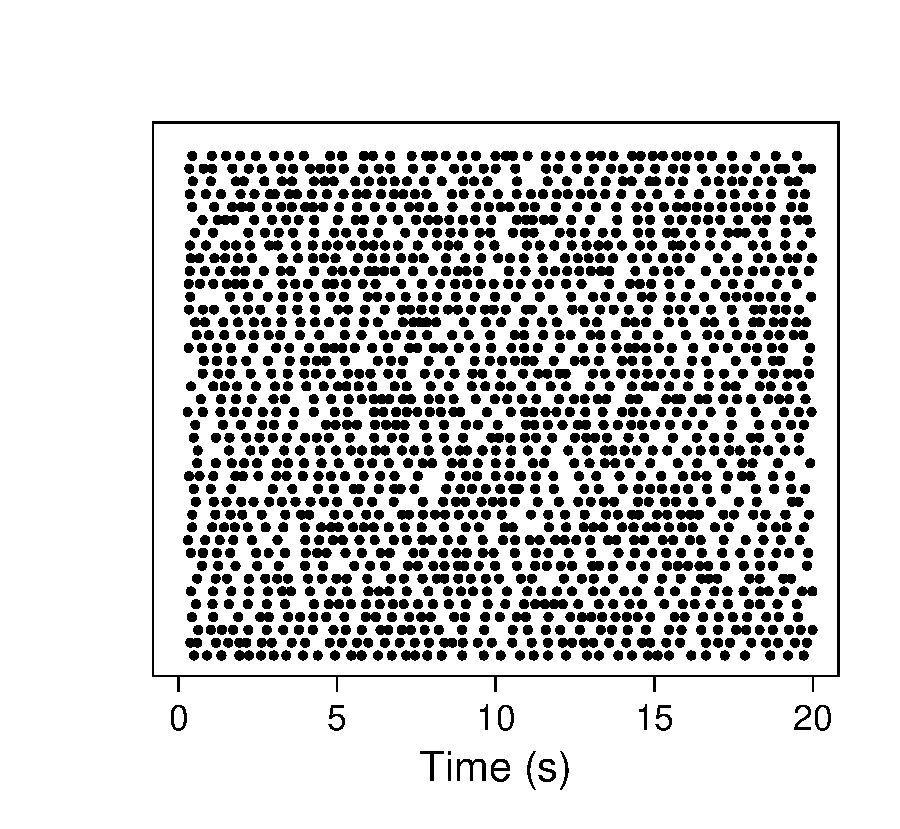
\includegraphics[scale = 0.42]{ConRastor} }} \qquad
\subfloat[]{{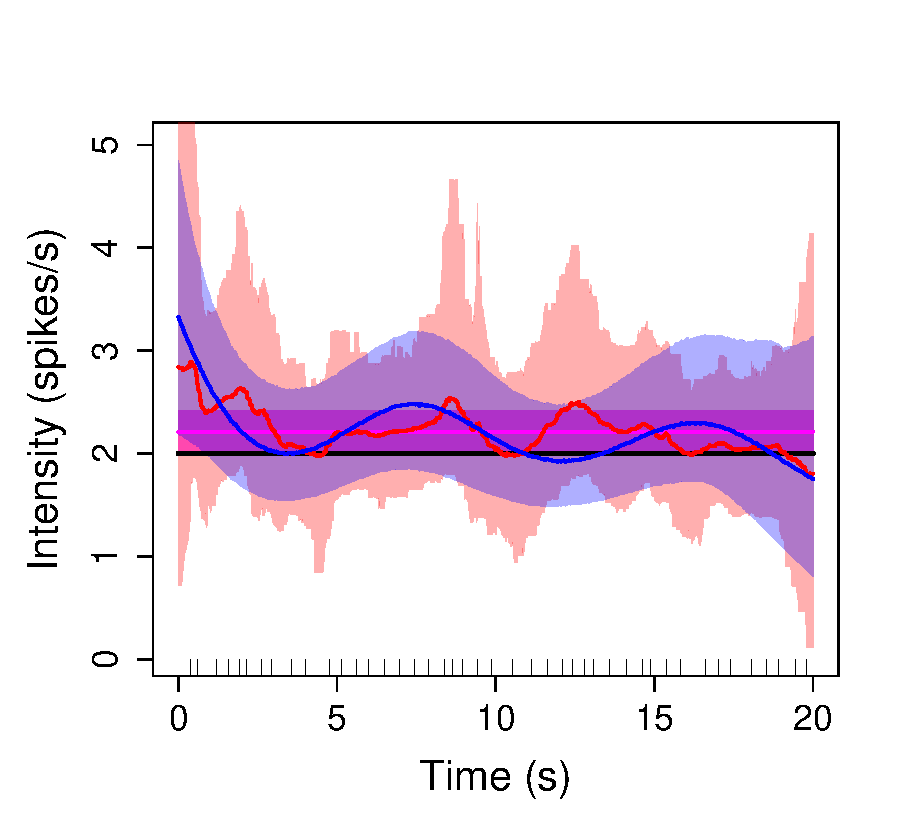
\includegraphics[scale = 0.42]{ConIntensity} }}  \\
\subfloat[]{{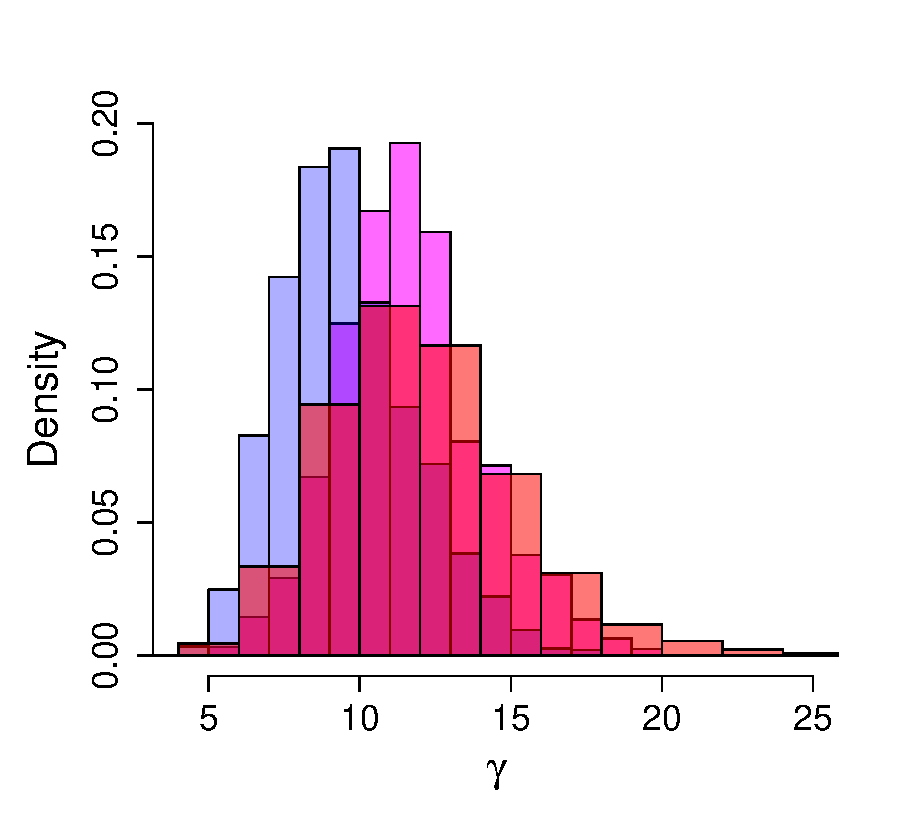
\includegraphics[scale = 0.42]{ConISIParam} }} \qquad
\subfloat[]{{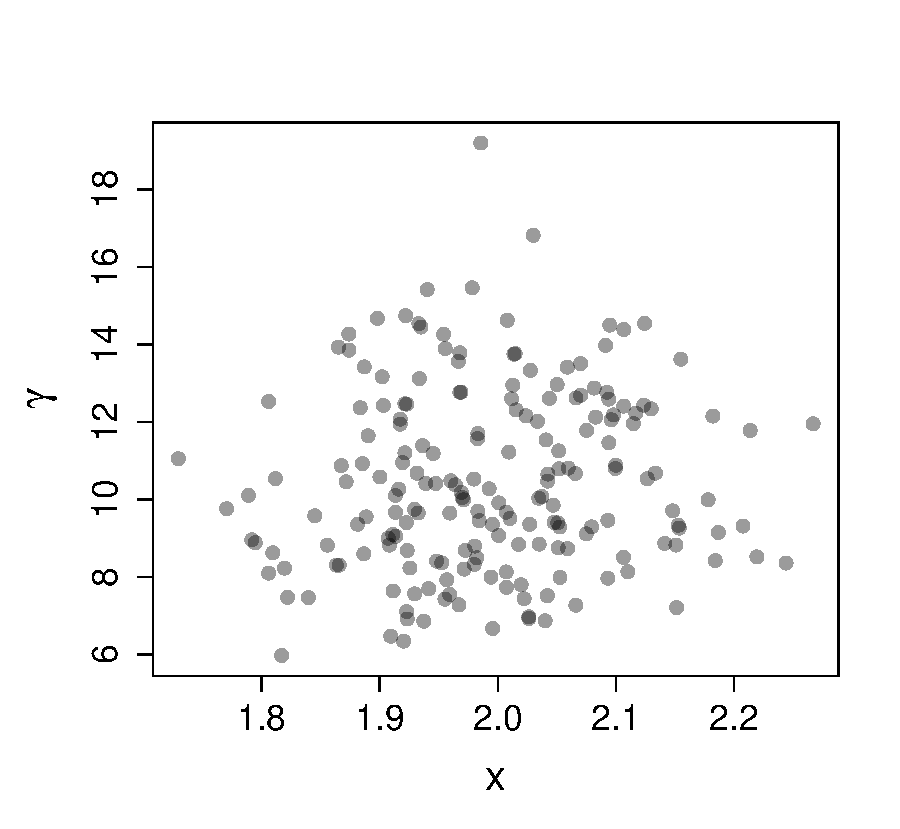
\includegraphics[scale = 0.42]{Conall} }}  \\
\end{center}     
\caption{Results from simulated data with constant intensity. (A) Rastor plot of 40 of the simulated spike sequences. (B) Posterior intensity function results for a single spike sequence, where the black line corresponds to the intensity the spikes were sampled from. In addition red, blue and magenta lines correspond to posterior intensity computed via PWC, GP and simple priors respectively, where the shaded areas correspond to the 95\% confidence regions. (C) Histogram of the posterior samples of the ISI parameter $\gamma$ for the same spike sequence as (B) where the colours represent the priors PWC (red), GP (blue) and simple (magenta). (D) Scatterplot of the MLEs for 200 spike sequences, where each dot corresponds to the MLE of a single spike sequence.}
\hrulefill
\label{fig:ResultsSimple}
\end{figure}

For the GP prior the inputs are: $T=20$, $M=6000$, $M_{\mathrm{burn}}=4000$, $\mathbf{t} = \{0,0.05,0.1, \dots, 20 \} $, $\omega = 0.01$, $\sigma^2_\theta = 1$ and $\sigma^2_l = 0.5$. 

Figure \ref{fig:ResultsSimple} (A) is a rastor plot of 40 simulated spike sequences.  In figure \ref{fig:ResultsSimple}(B,C) we have the posterior results for a single spike sequence, which can be seen as the rugs in (B). In (B) we show the posterior results for $x$ and in (C) the posterior results for $\gamma$. The colours red, blue and magenta correspond to the posterior results for PWC prior, GP prior and constant $x$ respectively. We find that the posterior distributions $x$ and $\theta$ are close to the model parameters ($x$ = 2, $\theta = 10$) the spike sequence was simulated from, as expected. Note that the intensities are all higher (~2.2) then the value simulated from (black line), this is due to the simulated spike sequence having 44 spikes.   Although not plotted the MLE values for the sequence were $x = 2.214$ and $\theta = 11.76$. Even though the PWC and GP prior allows for large changes in the intensity, we see that both remain approximately at 2.2, with slight variation due to variation in the ISIs. In (C) we plot the histograms of $\gamma$ generated by MCMC for the three priors, we see that whilst the distributions vary slightly all are centered around the true vale of $\gamma = 10$.  We have shown we recover parameter values for one sequence, however this could just be luck. To consolidate that we recover the model parameters we calculate the MLE for 200 spike sequences. In (D) we plot the MLEs for each individual spike sequence. We notice that the dots are scattered around the model parameters as expected. The variance of the dots around the model parameters we simulated from is due to the random nature of the simulated spikes. \\
    
 Consider a time-dependent intensity function, we choose $x(t) = 2 \cos(t/2)+1.1$, where the simulation time remains at 20s. We repeat the steps for the constant intensity above, simulating spike sequences and then fitting the model with these spike sequences. The inputs for inference remains the same for each prior. In figure \ref{fig:ResultsEx} (A) we show 40 simulated spike sequences with the time-dependent intensity function. The rastor plot clearly shows that the spiking intensity varies in time in a wave manner. In  figure \ref{fig:ResultsEx}(B,C) we show the posterior distribution for the intensity for two different spike sequences, shown as rugs in both plots. The black line corresponds to the intensity the spikes were simulated from. Both the posterior distributions from PWC (red) and GP (blue) priors recover the intensity. 


%%%%%%%%%%%%%%%%%%%%%%%%%%
%% Figure for time-varying intensity. 
\begin{figure}[t]
\hrulefill
\begin{center} 
\subfloat[]{{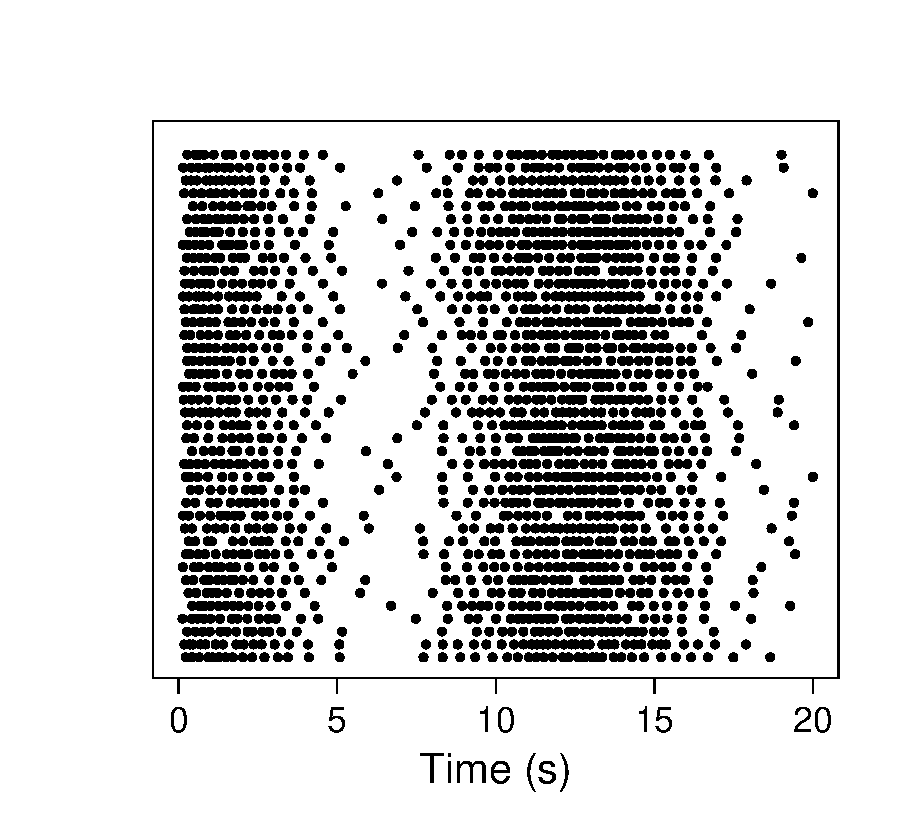
\includegraphics[scale = 0.42]{Ex_Rastor} }} \qquad
\subfloat[]{{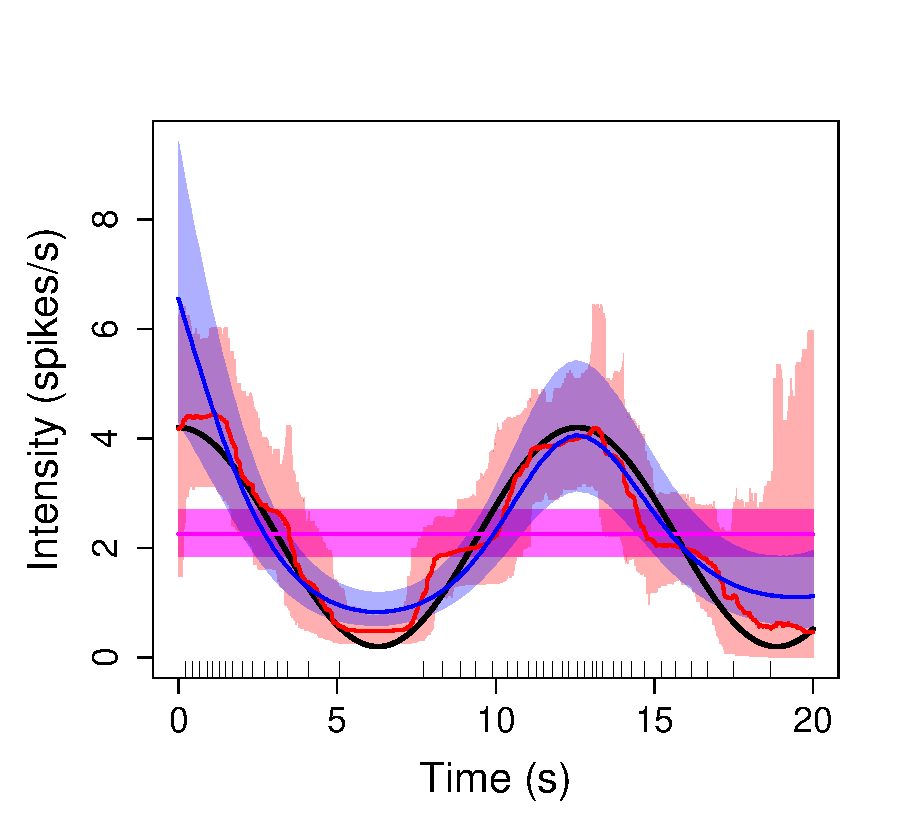
\includegraphics[scale = 0.42]{Ex_Int1} }}  \\
\subfloat[]{{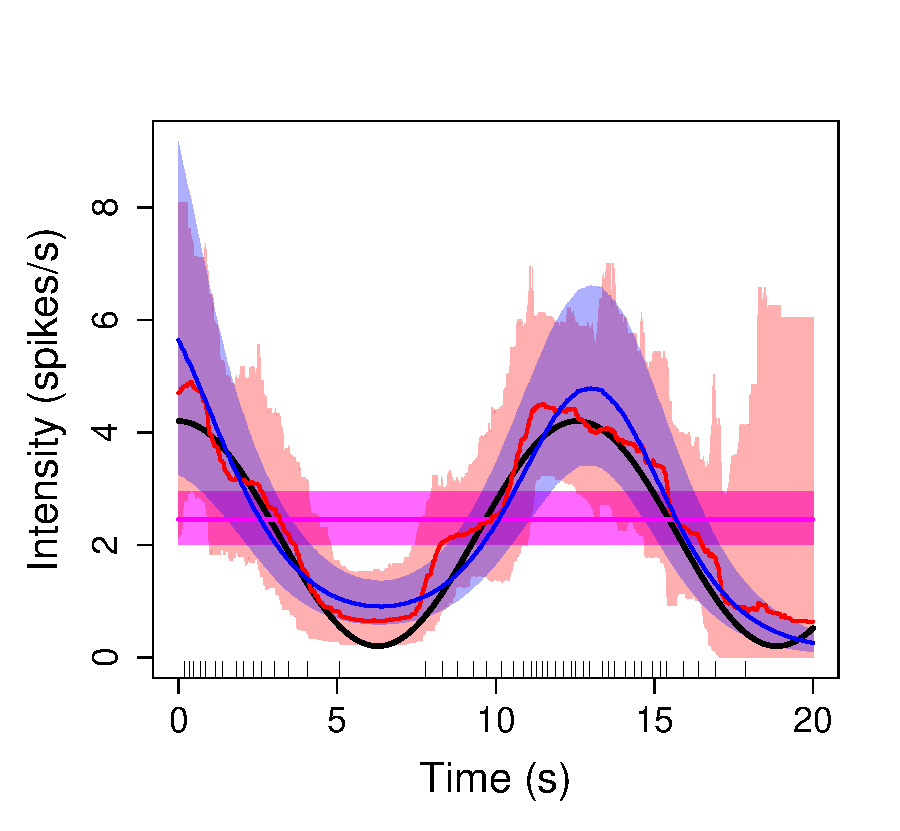
\includegraphics[scale = 0.42]{Ex_Int2} }} \qquad
\subfloat[]{{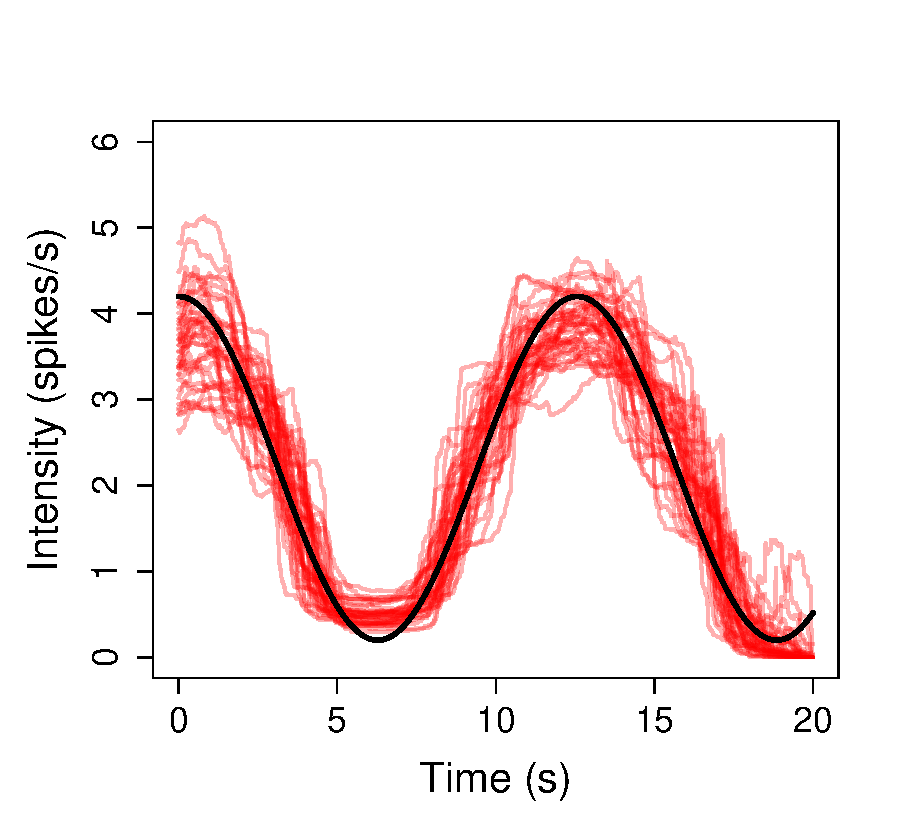
\includegraphics[scale = 0.42]{Ex_all} }}  \\
\end{center}     
\caption{Results from simulated data with time-varying intensity. (A) Rastor plot of 40 of the simulated spike sequences. (B,C) Posterior intensity function results for a single spike sequence, where the black line corresponds to the intensity the spikes were sampled from. In addition red, blue and magenta lines correspond to posterior intensity computed via PWC, GP and simple priors respectively, where the shaded areas correspond to the 95\% confidence regions.  (D) Scatterplot of average posterior intensity function for 40 spike sequences, where each red line corresponds to the mean posterior intensity function for a single spike sequence.      }
\hrulefill
\label{fig:ResultsEx}
\end{figure}




















%%%%%%%%%
%% NOT USED
%%%%%%%%%


%%%%%%%%%
%% The Likelihood.
%%%%%%%%%
%\subsection{Likelihood}
%Five different probability distributions were considered:
%\begin{itemize}
%
%\item Gamma:
%\begin{equation}
%p(y_i,y_{i-1}) = \frac{\gamma x(y_i)}{\Gamma (\gamma)} \big[ \gamma X(y_{i-1},y_i) \big]^{\gamma - 1} \mathrm{e}^{-\gamma X(y_{i-1},y_i) },
%\end{equation}
%where $\gamma > 0 $ denotes the shape parameter and $\Gamma$ is the Gamma function.  \\
%
%
%\item Inverse Gaussian:
%\begin{equation}
%p(y_i,y_{i-1}) = \frac{x(y_i) \sqrt{\lambda}}{\sqrt{2 \pi X(y_{i-1},y_i)^3}} \exp \bigg\{ -  \frac{\lambda (X(y_{i-1},y_i)- 1)^2}{2  X(y_{i-1},y_i)}\bigg\},
%\end{equation}
%where $\lambda > 0 $ is the variance parameter. The mean of the new IG is equal to $1/x$, the same as the Gamma distribution. \\
%
%
% \item Exponential:
%\begin{equation}
%p(y_i,y_{i-1}) = x(y_i) \mathrm{e}^{-X(y_{i-1},y_i)}.
%\end{equation}
%
%
%\item Log Normal:
%\begin{equation}
%p(y_i,y_{i-1}| \mu) = \frac{x(y_i)}{2X(y_{i-1},y_i)\sqrt{\mu \pi}} \exp\bigg\{ - \frac{(\log X(y_{i-1},y_i) + \mu)^2}{4 \mu} \bigg\}
%\end{equation}
%where $\mu >0$ is the shape parameter.  \\
%
%
%
%\item Weibull:
%\begin{equation}
%p(y_i,y_{i-1}| k, \lambda) = x(y_i) \frac{k}{\lambda} \bigg(\frac{X(y_{i-1}, y_i)}{\lambda} \bigg)^{k-1}  \exp \bigg\{ -\bigg( \frac{X(y_{i-1}, y_i)}{\lambda}\bigg)^k \bigg\} ,
%\end{equation}
%where $k, \lambda >0$ are the shape and scale parameters respectively. \\
%\end{itemize}


\end{document}
